\documentclass[12pt,vi]{mitthesis}
\usepackage{lgrind}
\usepackage{cmap}
\usepackage[T1]{fontenc}
\pagestyle{plain}
\usepackage{listings}
\usepackage{pdfpages}
\usepackage{hyperref}
\def\UrlBreaks{\do\/\do-}
\hypersetup{
    colorlinks=true,
    linkcolor=blue,
    filecolor=magenta,      
    urlcolor=cyan,
}
\usepackage{color}
\usepackage{graphicx}
\DeclareGraphicsExtensions{.pdf,.jpeg,.png,.jpg}
\lstset{language=bash}

\lstdefinestyle{BashInputStyle}{
  language=bash,
  basicstyle=\small\sffamily\color{yellow},
  numbers=left,
  numberstyle=\tiny,
  numbersep=3pt,
  frame=tb,
  columns=fullflexible,
  breaklines=true,
  backgroundcolor=\color{purple},
  linewidth=1\linewidth,
  xleftmargin=0.001\linewidth
}
\renewcommand*\contentsname{Sadržaj}
\renewcommand{\figurename}{Slika}
\begin{document}
\author{Dajan Bračković}
\department{Odsjek za Računarstvo i informatiku}
\degree{Master računarstva i informatike}
\degreemonth{Septembar}
\degreeyear{2020}
\thesisdate{Septembar ...., 2020}
\supervisor{Samir Ribić}{dr. sc.}
\chairman{Profesor dr. sc. Jasmin Velagić}{Dekan Elektrotehničkog fakulteta Univerziteta u Sarajevu}
\title{Modularizacija Linux SquashFS datotečnog sistema}

\maketitle
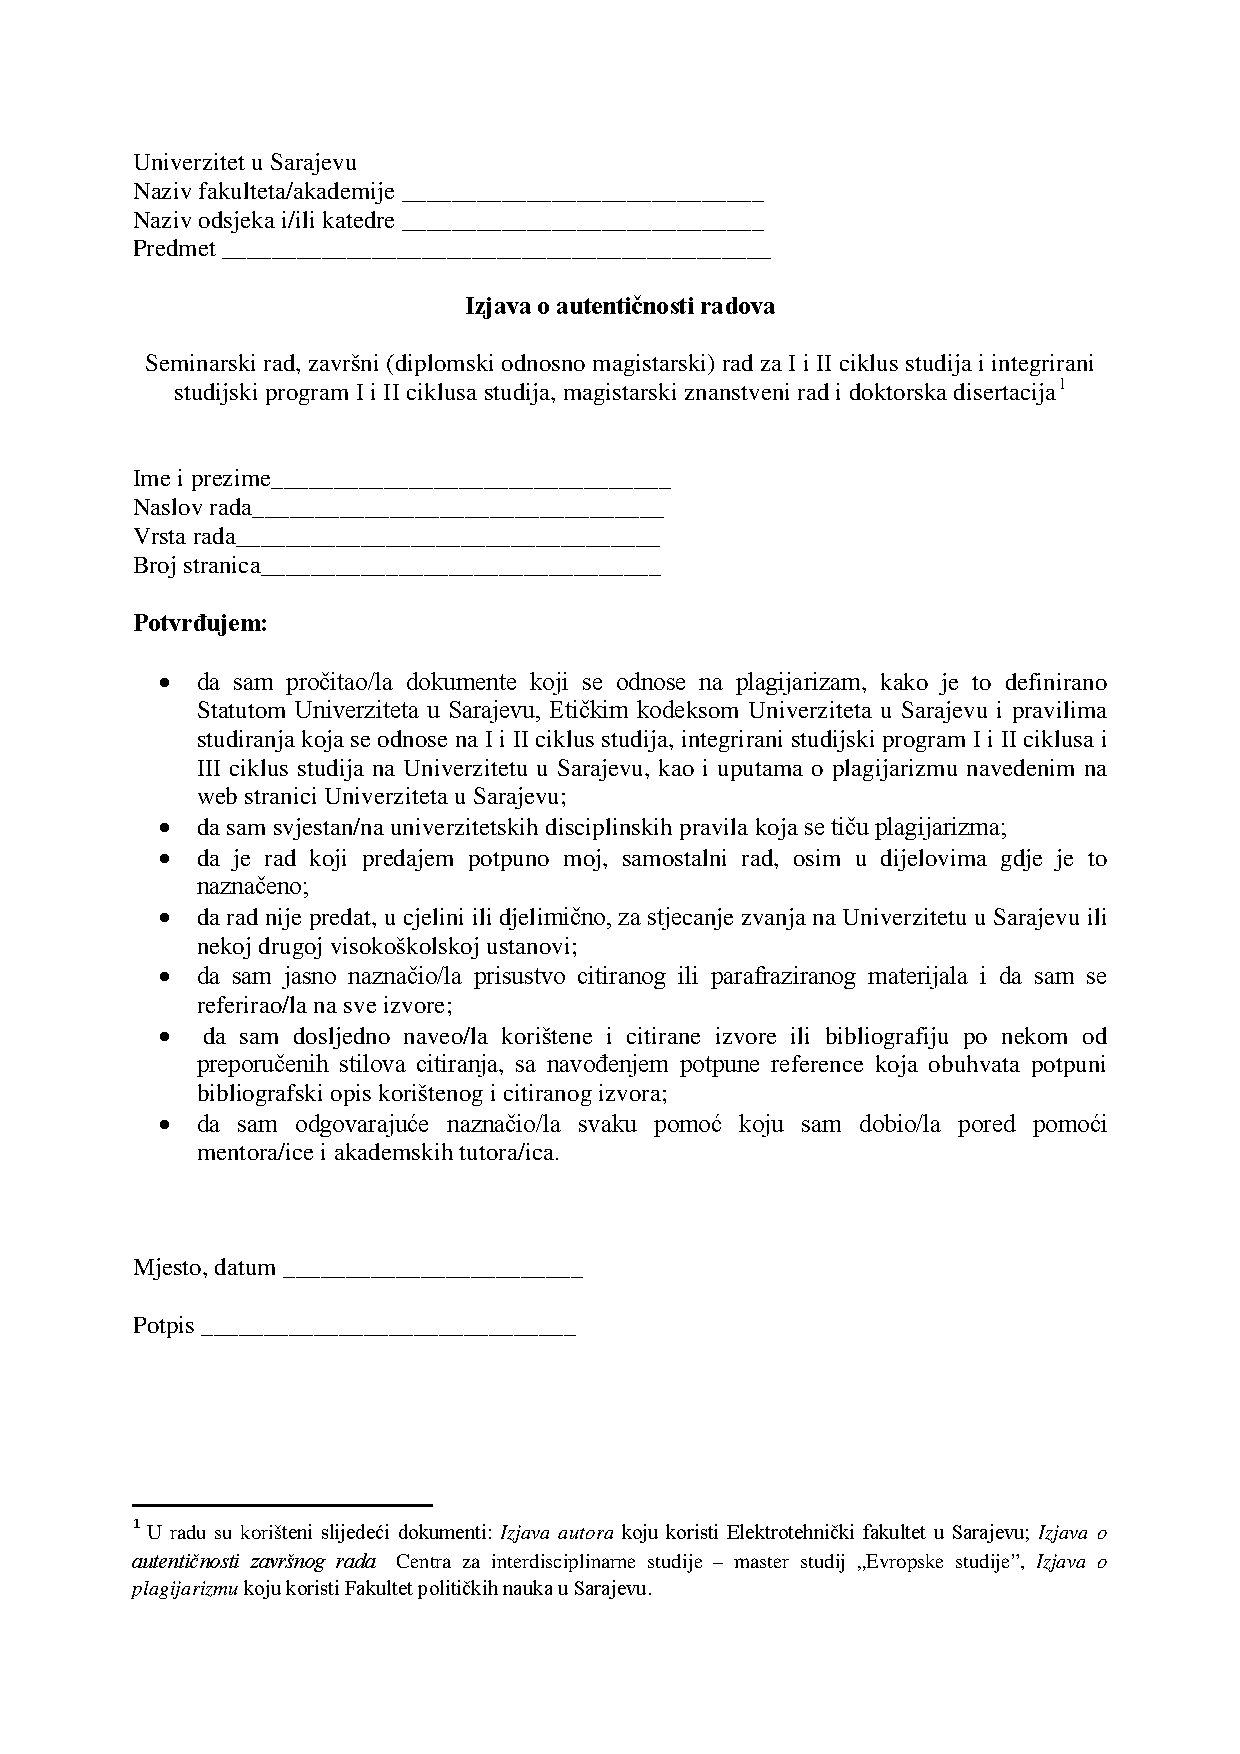
\includepdf[pages={1}]{izjava_autenticnosti.pdf}
\tableofcontents{}

\chapter*{Postavka rada}
\addcontentsline{toc}{chapter}{\numberline{}Postavka rada}
\noindent
\textbf{Tema:}\\
\indent
Modularizacija Linux SquashFS datotečnog sistema\\
\noindent
\textbf{Cilj:}\\
\indent
Primarni cilj je bolje upoznavanje sa Linux operativnim sistemom i sa načinom modifikacije instalacije Linux distribucije putem modularizacije squashfs datotečnog sistema.\\
Cilj izrade je kreiranje modifikovanih modula squashfs datotečnog sistema, koji imaju različite aplikacije predinstalirane. Na osnovu modula squashfs datotečnih sistema, kreirane su .iso datoteke.\\
Finalni produkti su 5 zasebnih .iso datoteka tijekom čije izrade je demonstriran proces modularizacije squashfs datotečnog sistema. Posljednja .iso datoteka, kreirana kao praktični dio rada, sadrži sve module unutar sebe, dok su prve četiri .iso datoteke kreirane svaka zasebno za jedan od modula. Ovaj primjer prikazuje razliku u kreiranju .iso datoteke u slučaju kada se unutar nje stave 4 .squashfs modula, u odnosu na način kreiranja .iso datoteke sa samo jednim .squashfs modulom.\\
\noindent
\textbf{Opis:}\\
\indent
Rad opisuje proces modularizacije squashfs datotečnog sistema. Pored toga opisani su termini i tehnologije korištene kroz proces modularizacije. Rad se ne ograničava striktno na opisivanje alata za kreiranje i manipuliranje .squashfs datotekama, nego i na sve aplikacije koje su instalirane kao zasebni moduli.\\
\indent
Rad spominje termine kao Ubuntu, LiveCD, Slax, NodeJS, MongoDB... te su oni opisani u sažetoj formi. Glavni fokus rada su procesi modularizacije i modifikacije squashfs datotečnog sistema, izrade i generisanja .iso datoteka. Napomena, da je generisanje .iso datoteke jedna komanda u komandnom interfejsu, stoga je to samo mali dio procesa, dok je većina procesa priprema i modifikacija datotečnog sistema. Generisanje .iso datoteke je posljednji korak izrade svakog od modula.

\chapter*{Sažetak}
\addcontentsline{toc}{chapter}{\numberline{}Sažetak}
\indent
U ovom poglavlju je sažeto opisan sadržaj rada i poglavlja koja slijede.\\
\indent
Uvodno poglavlje objašnjava pojmove poput live tj. žive distribucije, načina kreiranja live distribucija, te razloge njihove upotrebe.
Nakon toga su opisani datotečni sistemi, njihove vrste i detaljniji opis squashfs datotečnog sistema.
Zatim slijede kratka podpoglavlja o Slax/Nimblex/Ubuntu distribucijama, koje su jedne od popularnijih live distribucija, koje koriste squashfs datotečni sistem. Spomenuti su i neki od razloga zbog kojih se modifikuju instalacione .iso datoteke.\\
\indent
Sljedeće poglavlje je kratki opis sistemskih zahtjeva.\\
\indent
Poglavlje 'Priprema radnog okruženja' prikazuje listu potrebnih paketa za realizaciju modifikacije squashfs datotečnog sistema, kao i način instalacije ovih paketa.\\
\indent
Poglavlje 'Proces kreiranja zasebnih modula' sadrži više podpoglavlja. U cjelosti ovo poglavlje opisuje proces kreiranja 4 .iso datoteke a to su:\\
\indent
1. ubuntu-with-nodejs-18.04-amd64.iso\\
\indent
2. ubuntu-with-mongodb-18.04-amd64.iso\\
\indent
3. ubuntu-with-java-18.04-amd64.iso\\
\indent
4. ubuntu-with-chrome-18.04-amd64.iso\\
Finalni proizvodi praktičnog rada opisanog ovim poglavljem su .iso datoteke koje imaju predinstalirane neke od danas popularnih aplikacija u svijetu programiranja. Aplikacije su instalirane unutar zasebnih filesystem.squashfs modula, iz kojih su generisane 4 zasebne .iso datoteke. U ovom poglavlju se najviše referenciraju uputstva na \cite{ubuntuLiveCD} i \cite{custom-ubuntu-live}, koja se tiču redoslijeda izvršavanja komandi za modifikaciju Linux live distribucije.\\
\indent
U poglavlju 'Kreiranje više modula unutar jedne .iso datoteke' je fokus na generisanju jedne .iso datoteke koja sadrži 5 .squashfs modula unutar sebe. To su moduli: bazni, nodejs, mongodb, java i chrome. Opisuje se sličan proces kao u prethodnom poglavlju, uz nekoliko razlika. To su potreba pravljenja delta direktorija za svaki modul, generisanje status.diff datoteke, te kreiranje .iso datoteke koja sadrži 5 .squashfs modula. Kao usporedba sa prethodnim poglavljem u kojem su kreirane 4 .iso datoteke, svaka za jedan modul, u ovom poglavlju je kreirana jedna .iso datoteka sa 5 .squashfs datoteka, svaka za jedan od 4 modula + bazni modul.\\
\indent
Poglavlje 'Zaključaj' opisuje moguća poboljšanja i dorade. Kao primjer upotrebe modularizacije .squashfs datotečnog sistema navodi se mogućnost kreiranja modularne linux distribucije koja bi omogućavala korisniku odabir između KDE, GNOME, Xfce, LXDE grafičkih interfejsa, te mehanizam uključivanja/isključivanja željenog grafičkog interfejsa. Kao drugi primjer je opisana mogućnost primjene koncepta modularizacije .squashfs datotečnih sistema za kreiranje namjenskog operativnog sistema na Elektrotehničkom fakultetu Univerziteta u Sarajevu.

\chapter*{Abstract}
\addcontentsline{toc}{chapter}{\numberline{}Abstract}
\indent
This work is describing the process of modularization of Linux SquashFS filesystem. Modularization is performed by manual customization of packages in the live system, then extracting that customized system as a separate module.\\
\noindent
This thesis will show how to create 4 separate modules out of the same base image, which will be the ubuntu-18.04.4-desktop-amd64.iso.\\
\noindent
Also the thesis will show the process of integrating 4 separate modules inside a single ubuntu-18.04.4-desktop-amd64.iso image.\\
\noindent
We will be using the SquashFS tools to make the modifications inside the ubuntu-18.04.4-desktop-amd64.iso image.

\chapter*{Uvod}
\addcontentsline{toc}{chapter}{\numberline{}Uvod}
\section*{Live distribucija?}
\addcontentsline{toc}{section}{\numberline{}Live distribucija?}
\indent
Svaka .iso datoteka kreirana tokom izrade i pisanja rada je pokrenuta kao live distribucija unutar kvm-qemu emulatora. Zbog toga je u nastavku opisan pojam live distribucije.\\
\indent
Live distribucije\cite{wiki-livecd} omogućavaju korisniku da pokrene operativni sistem sa nekog eksternog uređaja kao što su CD/DVD, USB, HDD ili SSD (HDD i SSD se češće koriste kao eksterni diskovi na koje je u potpunosti instaliran operativni sistem), te da se operativni sistem učita u cjelosti u RAM memoriju. To omogućava upotrebu operativnog sistema bez potrebe da se isti instalira na interni disk računara.\\
\indent
Najčešće se koriste live CD/DVD ili USB distribucije.
Na ovaj način se može pokrenuti instanca operativnog sistema na računaru koji već ima prethodno instaliran operativni sistem, te nakon upotrebe ugasiti računar, i izvaditi USB/CD/DVD uređaj sa kog je pokrenut "živi" operativni sistem. Prilikom sljedećeg paljenja računara, biće pokrenut originalno instalirani operativni sistem.\\
Može se reći da su CD/DVD live distribucije sve manje i manje popularne zbog rasta upotrebe USB uređaja za pokretanje live distribucija.\\
\indent
Za razliku od live CD/DVD instalacija, podaci na USB uređaju mogu biti modificirani i dodatni podaci mogu biti upisani na uređaj. Korisnik može sa sobom u džepu nositi kompletan operativni sistem, aplikacije, konfiguracione datoteke i mnogo ličnih podataka.\\
\indent
Sa aspekta sigurnosti USB live distribucije imaju prednosti i mane. Svakako da je USB mnogo manji i stoga je lakše ga prenijeti i sakriti na neku sigurnu lokaciju, pri čemu se onemugućuje drugima da pristupe vašim podacima. Međutim svakako da ga je lakše izgubiti, pa su šifriranje podataka i rezervna kopija mnogo važniji nego u slučaju tradicionalnog desktop operativnog sistema.\\
\indent
Treba imati na umu da je pokretanje live instalacija na starijim mašinama koje nemaju podršku za USB 2.0 protokol, jako sporo.\\
Neke mašine ne dozvoljavaju pokretanje tj. "bootanje" sa USB uređaja, te je potrebno uključiti tu opciju unutar BOOT menadžera u BIOS-u.
\subsection*{Postupak kreiranja live USB}
\addcontentsline{toc}{subsection}{\numberline{}Postupak kreiranja live USB}
\indent
Postupak kreiranja live USB distribucije je sljedeći:\\
\indent
1. Uključivanje USB uređaja u računar\\
\indent
2. Preuzimanje instalacione datoteke, npr.\\fedora 32 \url{https://getfedora.org/en/workstation/download/}\\
ili npr. ubuntu 20.04 \url{https://ubuntu.com/download/desktop}\\
\indent
3. U Linux terminalu, tj. komandnom interfejsu, izvršavanje komande:
\begin{lstlisting}[style=BashInputStyle]
lsblk
\end{lstlisting}
\indent
Ispis bi trebao imati sadržaj sličan sljedećem:\\
\begin{figure}[!htb]
\centering
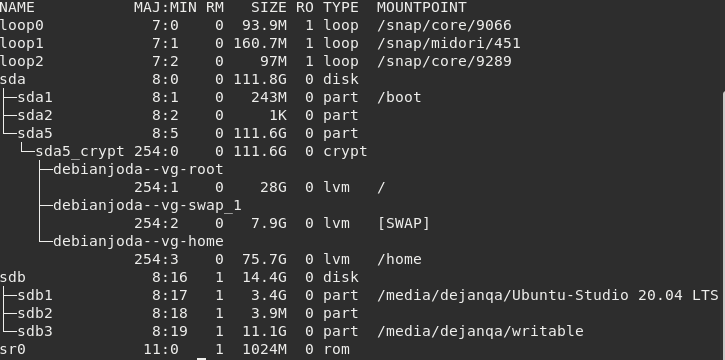
\includegraphics[width=\linewidth]{images/lsblkOutput.png}
\caption{Ispis lsblk komande}
\end{figure}
\indent
4. Slika iznad potvrđuje da je uključen USB uređaj. Komande navedene u odsječku ispod:
\begin{lstlisting}[style=BashInputStyle]
sudo umount /dev/sdb1
sudo umount /dev/sdb3
\end{lstlisting}
uklanjaju particije na USB uređaju koje imaju MOUNTPOINT.\\
\indent
5. Komanda:
\begin{lstlisting}[style=BashInputStyle]
sudo dd bs=4M if=path/home/user/downloads/ubuntu-20.04-amd64.iso of=/dev/sdb conv=fdatasync  status=progress
\end{lstlisting}
se izvršava duže vrijeme i podrazumijeva brisanje cijelog sadržaja na USB uređaju, pa korisnik treba biti svjestan te činjenice.\\
\indent
Nakon uspješnog izvršavanja dd komande je kreiran "live USB".\\
\indent
6. Ponovno pokretanje računara (restart) te "bootanje" sa uključenog USB uređaja na koji je instalirana .iso datoteka. Na većini računara za ulazak u boot meni je potrebno pritisnuti neku od F1->F12 tipki te odabrati opciju da računar "boot"-a sa USB uređaja.\\
\indent
7. Odabir opcije "Try Ubuntu without installing" pokreće ubuntu live distribuciju.

\subsection*{Upotrebe live distribucija}
\addcontentsline{toc}{subsection}{\numberline{}Upotrebe live distribucija}
\indent
Live distribucije imaju razne upotrebe:\\
\indent
1. Za instalaciju operativnih sistema na HDD/SSD\\
\indent
2. Za popravku i spašavanje podataka sa računara\\
\indent
3. Za kompjutersku forenziku\\
\indent
4. Za izlistavanje i testiranje hardvera\\
\indent
5. Za sigurnosno testiranje mreže\\
\indent
6. Za promjenu, krađu, probijanje šifri\\
\indent
7. Za skeniranje i odstranjivanje virusa i malvera\\
\indent
8. Za internet bankarstvo, kao namjenski konfigurisana platforma sa pojačanim sigurnosnim aspektima.\\
\indent
9. Za testiranje softvera...\\
\section*{Datotečni sistemi}
\addcontentsline{toc}{section}{\numberline{}Datotečni sistemi}
\indent
Datotečni sistemi\cite{tldp-guide} ("file systems" ili "filesystems")\cite{wiki-filesystem} su skupina metoda i podatkovnih struktura koje operativni sistem koristi radi vođenja evidencije o podacima na disku ili particiji diska. Datotečni sistem određuje način na koji su organizovani podaci na disku.\\
Prije nego što disk ili particija diska mogu biti upotrijebljeni kao datotečni sistem, datotečni sistem mora biti inicijaliziran na disk/particiju i strukture za čuvanje podataka trebaju biti upisane u disk. Ovaj proces se zove kreiranje datotečnog sistema.\\
Prije svega treba napomenuti da su Linux datotečni sistemi su slični UNIX datotečnim sistemima. Većina UNIX datotečnih sistema ima sličnu strukturu i uređenost. Glavni koncepti su "superblock" ili superblok, "inode" ili indeksni čvor\cite[str.~281]{operativni-sistemi}, "data block" ili blok podataka, "directory block" ili blok direktorija i "direction block" tj. blok pokazivač.\\
"Superblock" sadrži informacije o datotečnom sistemu uopćenito, npr. veličina datotečnog sistema. "Inode" ili indeksni čvor sadrži sve informacije o pojedinačnoj datoteci, izuzev njenog naziva. Nazim se smješta u direktorij zajedno sa rednim brojem indeksnog čvora.\\
Različiti operativni sistemi nemaju podršku za iste datotečne sisteme\cite{wiki-filesystem-comparison}\cite{filesystem-comparison}. Windows podržava NTFS\cite[str.~286]{operativni-sistemi}, dok Linux koristi uglavnom EXT2\cite[~302]{linux-bible}, EXT3\cite[~302]{linux-bible}, EXT4\cite[~302]{linux-bible}, ali i dosta drugih. Mac s druge strane HFS+.\\
FAT32 je stariji datotečni sistem razvijen od Microsoft-a, ali ga podržavaju i Linux i Windows operativni sistemi pa je nekad koristan za USB diskove koji se dijele između Windows-a i Linux-a.

\subsection*{SquashFS datotečni sistem}
\addcontentsline{toc}{subsection}{\numberline{}SquashFS datotečni sistem}
\indent
SquasFS\cite[str.~303]{linux-bible}\cite{squashfs-howto}\cite{squashfs-deployment} je kompresovani "read-only" file system. Squasfs kompresuje datoteke, indeksne čvorove i direktorije. Podržava blokove veličina između 4KiB i 1MiB.\\
\indent
SquashFS datotečni sistem je napisan od strane 	Phillip Lougher-a i Robert Lougher-a. 
Nekoliko algoritama za kompresiju su podržani kao gzip, LZMA i LZO.\\
Squashfs se koristi u Live CD verzijama Arch Linux-a, Debian-a, Fedora-e, Gentoo Linux-a, HoleOS-a, Salix-a, Ubuntu-a, Clonezilla-e, "embedded/ugradbenim" distribucijama kao što su "OpenWrt" i DD-WRT ruter firmware. Koriste ga i Chromecast i Android Nugat. AppImage koristi squasfs za generisanje "appimages".\\

\section*{Slax}
\addcontentsline{toc}{section}{\numberline{}Slax}
\indent
Slax\cite{slax-org}\cite{slax-wiki} je LiveCD Linux distribucija koju aktivno razvija Tomáš Matějíček. Na oficijelnoj stranici Slax operativnog sistema stoji opis "Vaš džepni operativni sistem".\\
\indent
Jedna od prednosti Slax operativnog sistema je jednostavnost modifikacije. Paketi mogu biti dodani i uklonjeni koristeći Slax module, koji su kompresovani "read-only" squasfs datotečni sistemi kompresovani pomoću LZMA algoritma.\\
Paketi mogu biti instalirani upotrebom apt paket menadžera, zatim se spašava modul sa .sb ekstenzijom, te se generiše slax.iso sa tim novokreiranim modulom.sb pomoću genslaxiso komande.\\
\subsection*{Primjer aktiviranja/deaktiviranja Slax modula}
\addcontentsline{toc}{subsection}{\numberline{}Primjer aktiviranja/deaktiviranja Slax modula}
\indent
Ispod su izlistane komande unutar Slax distribucije za instaliranje, aktiviranje, deaktiviranje modula sa firefox-esr(firefox-extended-support-release) paketom.
\begin{lstlisting}[style=BashInputStyle]
apt install firefox-esr
savechanges firefox.sb
genslaxiso slax.iso firefox.sb
slax activate firefox.sb
slax deactivate module.sb
\end{lstlisting}
\section*{NimbleX}
\addcontentsline{toc}{section}{\numberline{}NimbleX}
\indent
NimbleX\cite{NimbleX-wiki} je Linux distribucija optimizirana da se pokrene sa CD-a, USB-a ili direktno preko mreže. Karakteristika NimbleX-a je brzo boot-anje, i mala količina prostora na disku koju zauzima, s obzirom da je distribuiran sa KDE desktop okruženjem. NimbleX je jedinstven po svojoj web stranici koja dozvoljava korisnicima da generišu "boot-abilne" distribucije modifikovane putem browsera. NimbleX boot-a u otprilike duplo kraćem vremenskom roku od Ubuntu ili recimo Fedora distribucije.\\
NimbleX je bio na strani kritika zbog nedostatka instaliranih sigurnosnih softverskih paketa. Prvi put je objavljen 20-og oktobra 2004-te godine. Glavni inžinjer odgovoran za razvoj NimbleX-a je rumun Bogdan Rădulescu.\\
\indent
NimbleX koristi Linux kernel verziju 2.6. Predinstalirani grafički menadžer je KDE. Za kompjutere slabijih performansi može se podesiti i Fluxbox kao i Xfce kao grafički menadžer. Veličina instalacione datoteke NimblX distribucije je ispod 400MB, što nas navodi na logičan zaključak da NimbleX ne nudi previše grafičkih aplikacija, za dosta zadataka je neophodno koristiti terminal ili komandni interfejs. NimbleX nudi i instalacione datoteke manje veličine, npr. 100MB ili 69MB. Dodatne aplikacije se mogu instalirati putem grafičke aplikacije Gslapt, ili putem komande slapt-get u komandnom interfejsu. Na većim instalacionim NimbleX datotekama je predinstalirano mnoštvo korisnih aplikacija kao što su:\\
\indent
1. OpenOffice.org\\
\indent
2. Java\\
\indent
3. Python\\
\indent
4. Wine...
\section*{Ubuntu}
\addcontentsline{toc}{section}{\numberline{}Ubuntu}
Ubuntu\cite{ubuntu-wiki} je Linux distribucija zasnovana na Debian Linux distribuciji. Koristi isti paket menadžer kao i Debian. Ubuntu se oficijelno distribuira u 3 verzije:\\
\indent
1. Desktop\\
\indent
2. Server\\
\indent
3. Core - namijenjen za IoT uređaje.\\
\indent
Ubuntu verzije pristižu svakih 6 mjeseci, dok LTS verzije se objavljuju svake 2 godine. 23. Aprila 2020 je objavljena najnovija LTS verzija 20.04 pod nazivom "Focal Fossa".\\
\indent
Prvi put je objavljen 2004. godine. Ubuntu razvija kompanija Canonical, kao i čitav 'community' inžinjera koji svojim dobrovoljnim radom doprinose razvoju Ubuntu distribucija. Dobio je naziv iz jezika Nguni, koja u prevodu znači "čovječanstvo".\\
Pored gore navedenih distribucija Ubuntu-a, treba napomenuti da su jedno vrijeme bile u razvoju distribucije za pametne telefone i tablet uređaje, ali rad na ovim distribucijama je zaustavljen.\\
\indent
Ubuntu softverski paketi imaju istu .deb ekstenziju kao i kod Debian Linux distribucije. Ove dvije distribucije koriste i isti paket menadžer - apt.\\
\indent
Pored podjele Ubuntu distribucija na Desktop, Server i Core, Ubuntu pruža razne "Ubuntu flavours":\\
\indent
1. Kubuntu - Ubuntu distribucija sa KDE Plasma grafičkim okruženjem\\
\indent
2. Lubuntu - Ubuntu distribucija sa LXDE (Lightweight X11 Desktop Environment) grafičkim okruženjem, koje zahtjeva manje RAM memorije u odnosu na neka zahtjevnija grafička okruženja kao KDE ili GNOME\\
\indent
3. Xubuntu - Ubuntu distribucija sa podešenim Xfce grafičkim okruženjem, koje je također slično LXDE okruženju po pitanju zauzimanja resursa\\
\indent
4. Ubuntu Budgie - Ubuntu distribucija sa podešenim Budgie desktop okruženjem.\\
\indent
5. Ubuntu Kylin - Ubuntu distribucija namijenjena za kinesko tržište.\\
\indent
6. Ubuntu MATE - Ubuntu distribucija sa podešenim MATE desktop okruženjem.\\
\indent
7. Ubuntu Studio - Ubuntu distribucija namijenjena isključivo za multimedijsku produkciju. Dolazi sa Xfce gračifkim okruženjem. Jedna od najbitnijih karakteristika ove distribucije je "low-latency" jezgro sistema, koja je u osnovi standardno Linux jezgro, sa posebnom konfiguracijom koja dozvoljava stabilan rad audio aplikacija sa malim kašnjenjem. Ova distribucija dolazi sa instaliranim aplikacijama kao što su: Ardour, LMMS, Hydrogen, Audacity, JACK audio connection kit, Blender, GIMP, Krita, Kdenlive i mnogim drugim.
\section*{Zasto modifikovati instalacionu iso datoteku?}
\addcontentsline{toc}{section}{\numberline{}Zašto modifikovati instalacionu iso datoteku?}
Zašto uopće mijenjati instalacioni iso image operativnog sistema? Postoji nekoliko razloga:\\
1. Da bismo napravili svoju distribuciju mijenjajući postojeću iso datoteku\\
2. Da bismo predstavili određenu aplikaciju\\
3. Radi lokalizacije na određeni jezik\\
4. Da bismo uklonili određene softverske pakete\\
5. S ciljem dodavanja novih softverskih paketa\\
6. U svrhu ažuriranja softverkih paketa\\
7. Radi mijenjanja sistemske konfiguracije kao što su teme, ikone, fontovi, pozadina...\\
\\
Najlakši način modifikacije iso image-a baziranih na Ubuntu distribuciji je koristenjem "Ubuntu Customization Kit" alata. Međutim ovaj rad će obuhvatiti drugačiji princip, bez upotrebe "Ubuntu Customization Kit" alata.\\
Svaki od modula koji su kreirani su bazirani na istoj banoj .iso datoteci, ubuntu-18.04.4-desktop-amd64.iso. Modifikacijom istog dobit ćemo četiri modula raspoređena u različite .iso datoteke:\\ 
1. Modul NodeJS - ubuntu-with-nodejs-18.04-amd64.iso\\
2. Modul MongoDB - ubuntu-with-mognodb-18.04-amd64.iso\\
3. Modul Java - ubuntu-with-java-18.04-amd64.iso\\
4. Modul Google Chrome - ubuntu-with-google-chrome-18.04-amd64.iso\\
\indent
U posljednjem poglavlju prije zaključka je opisan proces kreiranja jedne .iso datoteke koja sadrži sve module skupa pod nazivom ubuntu-cjmn-18.04-amd64.iso. CJMN predstavlja skraćenicu za Chrome, Java, MongoDB, NodeJS aplikacije zajedno. Nije riječ o skraćenici općeprihvaćenoj nego je skraćenica iskorištena da bi naziv datoteke bio kraći.

\chapter*{Sistemski zahtjevi}
\addcontentsline{toc}{chapter}{\numberline{}Sistemski zahtjevi}
Lista hardverskih minimuma koje radna mašina treba da ispunjava su:\\
\indent
1. Najmanje 20GB slobodnog prostora na disku, poželjno bi bilo i više od 20GB, pogotovo ukoliko se pravi veći broj različitih modula.\\
\indent
2. Najmanje 2048MB RAM memorije i 4GB alocirane swap memorije.\\
\indent
3. Linux jezgro sa squashfs podrškom.\\
\indent
4. QEMU/KVM || VirtualBox || VMWare - bilo koji od ova 3 alata za testiranje kreiranih .iso datoteka.\\
\indent
5. genisoimage - paket za generisanje .iso datoteka\\

\chapter*{Priprema radnog okruženja}
\addcontentsline{toc}{chapter}{\numberline{}Priprema radnog okruženja}
\indent
Radno okruženje podrazumijeva radnu mašinu sa instaliranim Linux operativnim sistemom, kao i paketima squashfs-tools i genisoimage:
\begin{lstlisting}[style=BashInputStyle]
sudo apt-get install squashfs-tools genisoimage
\end{lstlisting}

\section*{SquashFS paket}
\addcontentsline{toc}{section}{\numberline{}SquashFS paket}
Paket squashfs-tools implementira 2 funkcije koje se koriste u ovom radu (\url{http://tldp.org/HOWTO/SquashFS-HOWTO/whatis.html}).
Radi se o funkcijama \textbf{mksquashfs} i \textbf{unsquashfs}. Prva od navedenih koristi se za kreiranje squashfs dateteke, dok se druga funkcija koristi za raspakivanje kompresovane squashfs datoteke.\\
SquashFS je moguće instalirati kao dodatak na Linux jezgro. Prema tome moguće ga je instalirati na različite Linux distribucije. Za Debian distribuciju njegov naziv je squashfs-tools.

\chapter*{Proces kreiranja zasebnih modula}
\addcontentsline{toc}{chapter}{\numberline{}Proces kreiranja zasebnih modula}
\indent
U ovom poglavlju je detaljno opisan proces kreiranja 4 modifikovane .iso datoteke od kojih svaka sadrži različite predinstalirane aplikacije. Svaka .iso datoteka u ovom slučaju predstavlja zasebni modul u svom završnom obliku.\\ 
Proces izrade zasebnih modula za svaki od modula je sličan, s tim da će se razlikovati nazivi direktorija, .iso datoteka i komandi za instaliranje aplikacija unutar raspakovanog .squashfs datotečnog sistema. Neki paketi se instaliraju direktno jednom komandom, dok je za neke druge potrebno vršiti dodatne konfiguracije.
\newpage
\section*{Modul NodeJS}
\addcontentsline{toc}{section}{\numberline{}Modul NodeJS}
\indent
NodeJS\cite{nodejs-wiki} je platforma "otvorenog koda" za izvršavanje JavaScript programa izvan okruženja mrežnog pretraživača. Neovisna je od vrste operativnog sistema i može se instalirati na Windows/Linux i MacOS operativne sisteme. JVM(JavaVirtualMachine), JRE(JavaRuntimeEnvironment) i JDK(JavaDevelopmentKit) zajedno predstavljaju sličnost sa NodeJS-om, ali za Java programski jezik. Može se reći da NodeJS objedinjuje sve te stvari u jedan koncept, ali za JavaScript programski jezik.\\
NodeJS ima "event-driven" baziranu arhitekturu koja omogućava asinhroni ulaz/izlaz informacija. To ga čini pogodnim za razvijanje web aplikacija koje imaju mnoštvo ulaznih/izlaznih operacija, kao i za razvoj mrežnih aplikacija za rad u realnom vremenu i igrica za mrežne pretraživače.\\
Prirodno NodeJS podržava samo JavaScript programski kod. Međutim podržava i programske jezike koji se daju kompajlirati u JavaScript. To su CoffeeScript, Dart, TypeScript, ClojureScript.\\
NodeJS se najčešće koristi za razvijanje WebServer-a. Jedna od bitnih razlika između NodeJS-a i PHP-a je ta što kod PHP-a većina funkcija blokira izvršavanje naredne funkcije dok se ne izvrši u potpunosti, dok su funkcije u NodeJS-u neblokirajuće te se mogu izvršavati paralelno, te na osnovu "callback" funkcije signaliziraju uspješno izvršenje ili grešku.\\
NodeJS je napravljen na osnovu Google V8 JavaScript programskog okruženja, koji prvenstveno napravljen za upotrebu u Google Chrome i Chromium pretraživačima.

\subsection*{Kreiranje direktorija potrebnih za rad - NodeJS modul}
\addcontentsline{toc}{subsection}{\numberline{}Kreiranje direktorija potrebnih za rad - NodeJS modul}
\noindent
NodeJS modul je kreiran od istog baznog modula kao i svi ostali moduli. To je ubuntu-18.04.4-desktop-amd64.iso datoteka. Direktorij livecdtmp je kreiran kao korijenski direktorij u koji su smješteni svi poddirektoriji i datoteke tijekom praktičnog rada:
\begin{lstlisting}[style=BashInputStyle]
mkdir ~/squashfs/livecdtmp
mkdir ~/squashfs/livecdtmp/isoimgs
mv ~/Downloads/ubuntu-18.04.4-desktop-amd64.iso ~/squashfs/livecdtmp/isoimgs
cd ~/squashfs/livecdtmp
\end{lstlisting}

\noindent
Na mnt direktorij unutar livecdtmp direktorija je montirana ubuntu-18.04.4-desktop-amd64.iso datoteka:
\begin{lstlisting}[style=BashInputStyle]
mkdir mnt
sudo mount -o loop ./isoimgs/ubuntu-18.04.4-desktop-amd64.iso mnt
\end{lstlisting}

\noindent
U direktorij extract-cd u je kopiran mnt direktorij izostavljajući filesystem.squashfs datoteku iz mnt/casper direktorija:
\begin{lstlisting}[style=BashInputStyle]
mkdir extract-cd
sudo rsync --exclude=/casper/filesystem.squashfs -a mnt/ extract-cd
\end{lstlisting}

\subsection*{unsquashfs filesystem.squashs datoteke - NodeJS modul}
\addcontentsline{toc}{subsection}{\numberline{}unsquashfs filesystem.squashfs datoteke - NodeJS modul}
\indent
Funkcija unsquashfs iz squashfs-tools paketa omogućava raspakivanje filesytem.squashfs direktorija. Rezultat unsquashfs funkcije je squashfs-root direktorij te je on kopiran u edit direktorij. Direktorij edit je u nastavku rada iskorišten da se unutar njega instaliraju nodejs paketi:
\begin{lstlisting}[style=BashInputStyle]
sudo unsquashfs mnt/casper/filesystem.squashfs
sudo mv squashfs-root/ edit
\end{lstlisting}

\subsection*{Konfiguracija paketa za chroot okruženje - NodeJS modul}
\addcontentsline{toc}{subsection}{\numberline{}Konfiguracija paketa za chroot okruženje - NodeJS modul}
\indent
Zbog potrebe za mrežnom konekcijom unutar edit direktorija neophodno je kopiranje sadržaja resolv.conf\cite[str.~809, str.~186]{linux-bible} iz sistema domaćina unutar edit direktorija:
\begin{lstlisting}[style=BashInputStyle]
sudo gedit edit/etc/resolv.conf
\end{lstlisting}
Kopirani sadržaj mora biti spremljen:\\
(\textit{nameserver 1.1.1.1 \\
nameserver 8.8.8.8}).\\
\noindent
Isto važi i za etc/hosts\cite[str.~186]{linux-bible} datoteku:
\begin{lstlisting}[style=BashInputStyle]
sudo gedit edit/etc/hosts
\end{lstlisting}
Također neophodno je kopiranje sadržaja iz /etc/hosts datoteke na sistemu domaćinu unutar edit/etc/hosts datoteke:
\begin{lstlisting}
127.0.0.1	localhost
127.0.1.1	debianjoda.joda.net	debianjoda
\end{lstlisting}

\noindent
Konfiguracija edit/dev direktorija je neophodna prije izvršavanja chroot komande koja otvara okruženje gdje se u nastavku instaliraju NodeJS paketi:
\begin{lstlisting}[style=BashInputStyle]
sudo mount --bind /dev/ edit/dev
sudo chroot edit
mount -t proc none /proc
mount -t sysfs none /sys
mount -t devpts none /dev/pts
\end{lstlisting}
Napomena da brisanje edit direktorija može učiniti sistem domaćin neupotrebljivim, ukoliko se ne uradi čišćenje u edit direktoriju nakon instalacije paketa.\\
\noindent
Podešavanje sistemskih varijabli unutar edit direktorija:
\begin{lstlisting}[style=BashInputStyle]
export HOME=/root
export LC_ALL=C
\end{lstlisting}

\subsection*{Instalacija nodeJS paketa unutar chroot okruženja}
\addcontentsline{toc}{subsection}{\numberline{}Instalacija nodeJS paketa unutar chroot okruženja}
\indent
Za ispis svih instaliranih paketa:
\begin{lstlisting}[style=BashInputStyle]
dpkg-query -W --showformat='\${Installed-Size}\t\${Package}\n' | sort -nr | less
\end{lstlisting}

\noindent
Instalacija NodeJS paketa unutar chroot okruženja\cite{nodejs-howto}
\begin{lstlisting}[style=BashInputStyle]
apt-get update
apt-get install curl
curl -sL https://deb.nodesource.com/setup_13.x | sudo -E bash -
apt-get install -y nodejs
\end{lstlisting}

\noindent
Čišćenje koje je neophodno unutar "chroot" okruženja:
\begin{lstlisting}[style=BashInputStyle]
apt-get clean
rm -rf /tmp/* ~/.bash_history
rm -rf /tmp/* ~/.bashrc
rm /var/lib/dbus/machine-id
rm /sbin/initctl
dpkg-divert --rename --remove /sbin/initctl
umount /proc || umount -lf /proc
umount /sys
umount /dev/pts
umount /dev
exit
\end{lstlisting}

\noindent
Ponovno generisanje filesystem.manifest datoteke:
\begin{lstlisting}[style=BashInputStyle]
sudo chmod +w extract-cd/casper/filesystem.manifest
sudo su
chroot edit dpkg-query -W --showformat='${Package} ${Version}\n' > extract-cd/casper/filesystem.manifest
exit
sudo cp extract-cd/casper/filesystem.manifest extract-cd/casper/filesystem.manifest-desktop
sudo sed -i '/ubiquity/d' extract-cd/casper/filesystem.manifest-desktop
sudo sed -i '/casper/d' extract-cd/casper/filesystem.manifest-desktop
\end{lstlisting}

\subsection*{Generisanje filesystem.squashfs datoteke - NodeJS modul}
\addcontentsline{toc}{subsection}{\numberline{}Generisanje filesystem.squashfs datoteke - NodeJS modul}
\noindent
Funkcija iz squashfs-tools, mksquashfs, omogućava kompresovanje edit direktorija u novu filesystem.squashfs datoteku. Ova filesystem.squashfs datoteka sadrži instalirane NodeJS pakete i datoteke. U kodu ispod su navedene 3 primjera mksquashfs funkcije, pri čemu prva (komanda na liniji 2) daje najslabiju kompresiju, ali je najbrža. Druga komanda se duže izvršava ali je veći procenat kompresije u odnosu na prvu komandu. Dok je kod treće komande procenat kompresije najveći, a vrijeme izvršenja najduže:
\begin{lstlisting}[style=BashInputStyle]
sudo rm extract-cd/casper/filesystem.squashfs
sudo mksquashfs edit extract-cd/casper/filesystem.squashfs -nolzma 
sudo mksquashfs edit extract-cd/casper/filesystem.squashfs -b 1048576
sudo mksquashfs edit extract-cd/casper/filesystem.squashfs -comp xz -e edit/boot
\end{lstlisting}

\noindent
Ažuriranje filesystem.size datoteke se vrši u odnosu na edit direktorij:
\begin{lstlisting}[style=BashInputStyle]
sudo su
printf $(du -sx --block-size=1 edit | cut -f1) > extract-cd/casper/filesystem.size
exit
\end{lstlisting}

\subsection*{Generisanje Ubuntu .iso image sa nodeJS modulom}
\addcontentsline{toc}{subsection}{\numberline{}Generisanje Ubuntu .iso image sa nodeJS modulom}
\noindent
Generisanje .iso datoteke je urađeno unutar extract-cd direktorija. Prije upotrebe genisoimage funkcije za generisanje .iso datoteke izvršena je nekolicina konfiguracijskih modifikacija.
Jedna od modifikacija je ažuriranje md5sum.txt datoteke:
\begin{lstlisting}[style=BashInputStyle]
cd extract-cd
sudo rm md5sum.txt
find -type f -print0 | sudo xargs -0 md5sum | grep -v isolinux/boot.cat | sudo tee md5sum.txt
\end{lstlisting}
\noindent
Druga modifikacija prije pozivanja genisoimage je upisivanje naziva 'Ubuntu with NodeJS 18.04.4 LTS "Bionic Beaver" - Release amd64' u polje DISKNAME unutar README.diskdefines datoteke:
\begin{lstlisting}[style=BashInputStyle]
sudo gedit extract-cd/README.diskdefines
\end{lstlisting}

\noindent
Za generisanje .iso datoteke koja sadrži NodeJS modul je iskorištena funkcija genisoimage. Neke Linux distribucije nude mkisofs funkciju, umjesto genisoimage funkcije:
\begin{lstlisting}[style=BashInputStyle]
sudo genisoimage -D -r -V "$IMAGE_NAME" -cache-inodes -J -l -b isolinux/isolinux.bin -c isolinux/boot.cat -no-emul-boot -boot-load-size 4 -boot-info-table -o ../ubuntu-with-nodejs-18.04-amd64.iso .
\end{lstlisting}

\subsection*{Pokretanje .iso datoteke pomoću KVM biblioteke}
\addcontentsline{toc}{subsection}{\numberline{}Pokretanje iso datoteke pomoću KVM biblioteke}
\indent
Za pokretanje kreirane .iso datoteke iskorišten je KVM alat. Najprije je kreiran virtuelni tvrdi disk pomoću qemu-img komande.
\begin{lstlisting}[style=BashInputStyle]
cd ~
qemu-img create ubuntunodejs.img 5G
\end{lstlisting}

\noindent 
Modulje pokrenut pomoću KVM-a:
\begin{lstlisting}[style=BashInputStyle]
sudo kvm -hda ubuntunodejs.img -cdrom ~/zavrsni/livecdtmp/ubuntu-with-nodejs-18.04-amd64.iso -boot d -m 2048
\end{lstlisting}

\subsection*{Rezultat Modul NodeJS}
\addcontentsline{toc}{subsection}{\numberline{}Rezultat Modul NodeJS}
\begin{figure}[!htb]
\centering
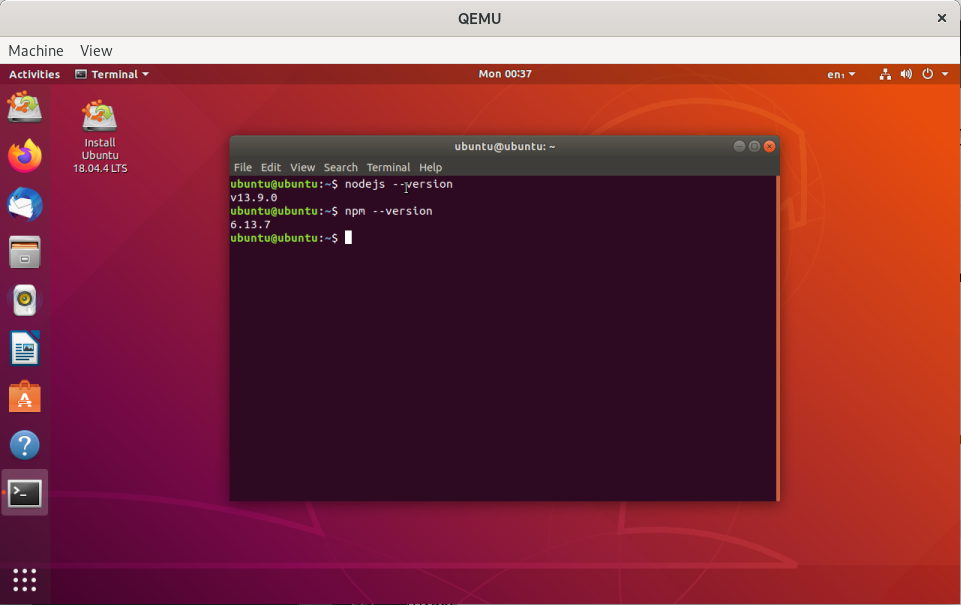
\includegraphics[width=\linewidth]{images/ModulNodeJSUbuntu.png}
\caption{ubuntu-with-nodejs-18.04-amd64.iso}
\end{figure}
\indent
Demonstrirana je upotreba NodeJS-a kreiranjem jednostavne mrežne aplikacije unutar novokreirane žive Ubuntu distribucije\cite{nodejs-helloworld-sample}.\\
Unutar pokrenute žive distribucije sa preidnstaliranim NodeJS bibliotekama pokrenuta je mrežna aplikacija putem NodeJS-a na vrlo jednostavan način:
\begin{lstlisting}[style=BashInputStyle]
git clone https://github.com/Azure-Samples/nodejs-docs-hello-world
cd nodejs-docs-hello-world
npm start
\end{lstlisting}
Potvrda da je mrežna aplikacija pokrenuta je server koji je pokrenut i može se provjeriti u mrežnom pregledniku na "URL"-u:
\begin{lstlisting}[style=BashInputStyle]
http://localhost:1337
\end{lstlisting}
Za potrebe rada nije rađena modifikacija ove mrežne aplikacije, ali moguće je iskoristiti aplikaciju kao bazu za nadograđivanje po želji. HTTP mrežni server se kreira unutar index.js datoteke te bi početna modifikacija mogla biti nadogradnja ove datoteke sa dodatnim funkcionalnostima.
\begin{figure}[!htb]
\centering
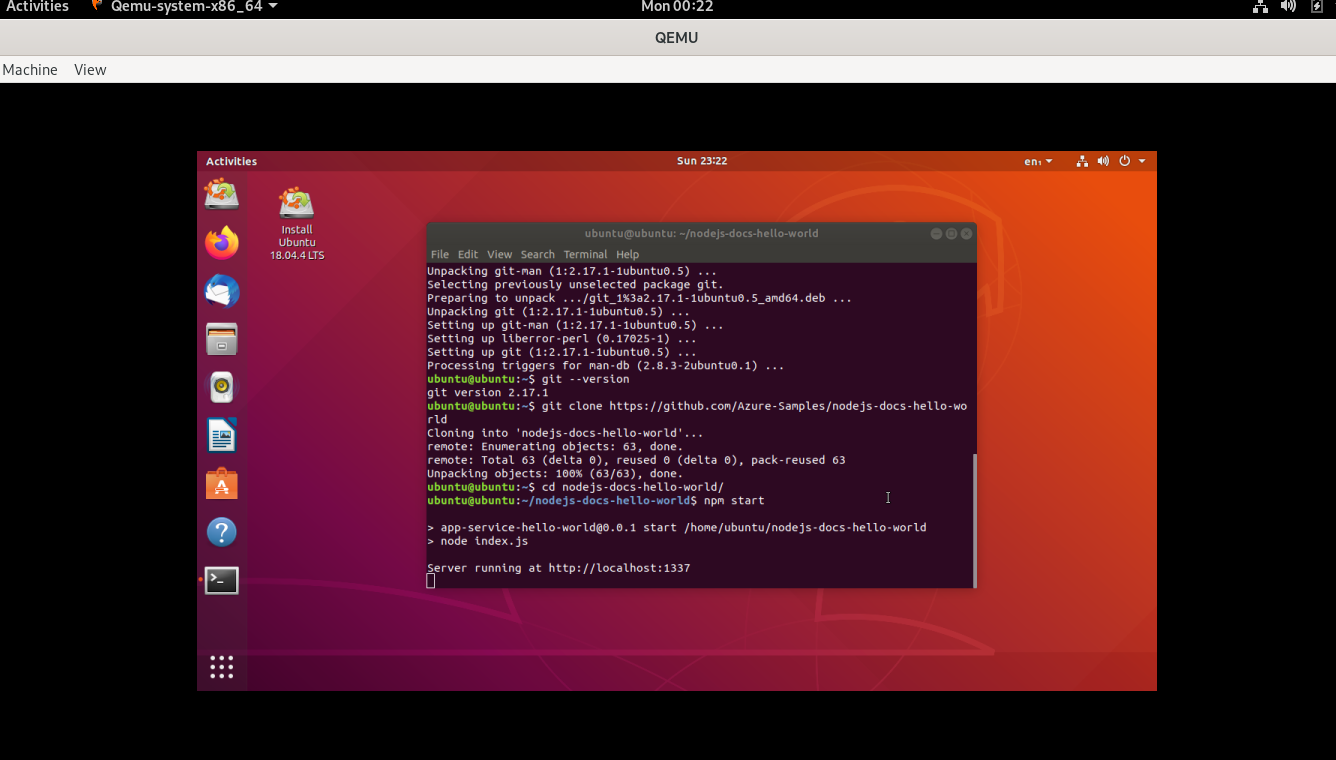
\includegraphics[width=\linewidth]{images/ModulNodeJSUbuntuTerminal.png}
\caption{Pokretanje NodeJS hello-world aplikacije}
\end{figure}
\begin{figure}[!htb]
\centering
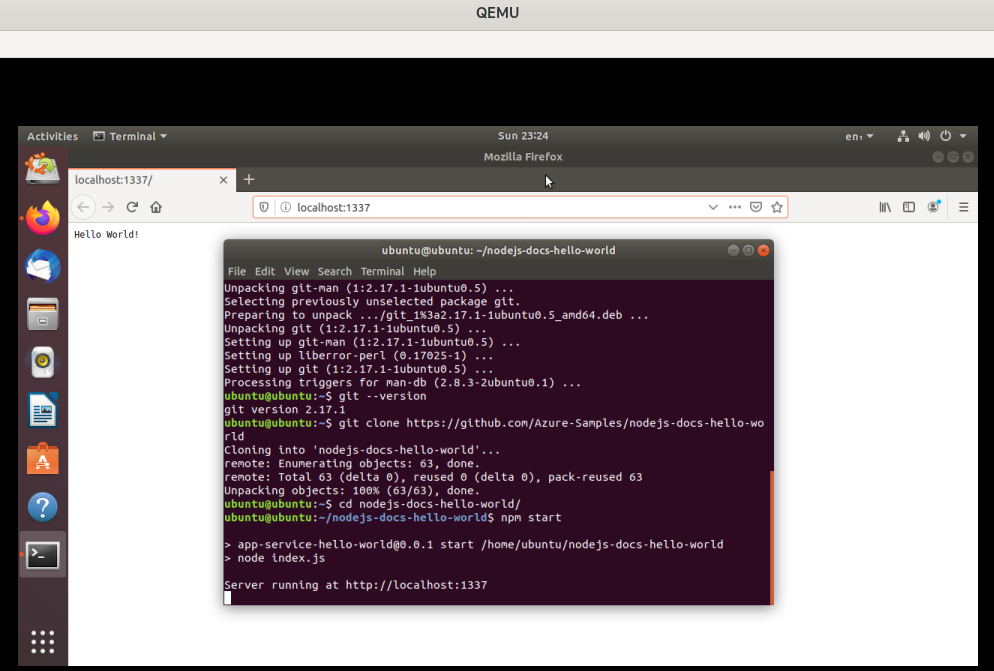
\includegraphics[width=\linewidth]{images/ModulNodeJSUbuntu1.png}
\caption{NodeJS hello-world aplikacija pokrenuta}
\end{figure}
\section*{Modul MongoDB}
\addcontentsline{toc}{section}{\numberline{}Modul MongoDB}
MongoDB je nerelaciona baza podataka napisana u C++ programskom jeziku. Koristi JSON format za spremanje podataka.\\
To je čini pogodnom za povezivanje sa NodeJS bibliotekama, čiji je modul već napraviljen u prethodnom paragrafu.\\
Postupak kreiranja ovog modula je gotovo identičan postupku kreiranja NodeJS modula, izuzev dijela u kojem se vrši instaliranje novih paketa unutar raspakovanog squashfs datotečnog sistema.
\subsection*{Kreiranje direktorija potrebnih za rad - MongoDB modul}
\addcontentsline{toc}{subsection}{\numberline{}Kreiranje direktorija potrebnih za rad - MongoDB modul}
\indent
Za potrebe kreiranja .iso datoteke za predinstaliranim MongoDB paketima kreiran je novi extract-mongodb-cd direktorij.
\begin{lstlisting}[style=BashInputStyle]
cd ~/squashfs/livecdtmp
sudo mount -o loop ./isoimgs/ubuntu-18.04.4-desktop-amd64.iso mnt
mkdir extract-mongodb-cd
sudo rsync --exclude=/casper/filesystem.squashfs -a mnt/ extract-mongodb-cd
\end{lstlisting}
\subsection*{unsquashfs filesystem.squashs datoteke - MongoDB modul}
\addcontentsline{toc}{subsection}{\numberline{}unsquashfs filesystem.squashfs datoteke - MongoDB modul}
\noindent
Raspakivanje filesystem.squashfs direktorija može potrajati par minuta:\\
\begin{lstlisting}[style=BashInputStyle]
sudo unsquashfs mnt/casper/filesystem.squashfs
\end{lstlisting}
Rezultat unsquashfs komande je squashfs-root direktorij koji je iskopiran u edit-mongodb direktorij:
\begin{lstlisting}[style=BashInputStyle]
sudo mv squashfs-root/ edit-mongodb
\end{lstlisting}
\subsection*{Konfiguracija paketa za chroot okruženje - MongoDB modul}
\addcontentsline{toc}{subsection}{\numberline{}Konfiguracija paketa za chroot okruženje - MongoDB modul}
\noindent
Datoteka resolv.conf unutar edit direktorija je ažurirana da bi se omogućila mrežna konekcija unutar chroot okruženja:
\begin{lstlisting}[style=BashInputStyle]
sudo gedit edit-mongodb/etc/resolv.conf
\end{lstlisting}
Sadržaj koji je unesen u resolv.conf datoteku:\\
(\textit{nameserver 1.1.1.1 \\
nameserver 8.8.8.8}).\\
\noindent
Iz /etc/hosts datoteke iz sistema domaćina sadržaj je iskopiran u edit-mongodb/etc/hosts datoteku:
\begin{lstlisting}[style=BashInputStyle]
sudo gedit edit-mongodb/etc/hosts
\end{lstlisting}
Novi sadržaj hosts datoteke:
\begin{lstlisting}
127.0.0.1	localhost
127.0.1.1	debianjoda.joda.net	debianjoda
\end{lstlisting}
\noindent
Neophodno je izvršiti chroot u edit-mongodb direktorij. U chroot okruženju će se instalirati MongoDB paketi. I u ovom slučaju ukoliko dođe do brisanja edit direktorija za mongodb, kojem je dat naziv edit-mongodb, sistem domaćin bi mogao postati neupotrebljiv. Tako da je prije brisanja neophodno izvršiti čišćenje, nakon instaliranja MongoDB paketa:
\begin{lstlisting}[style=BashInputStyle]
sudo mount --bind /dev/ edit-mongodb/dev
sudo chroot edit-mongodb
mount -t proc none /proc
mount -t sysfs none /sys
mount -t devpts none /dev/pts
\end{lstlisting}

\noindent
Izvršena je konfiguracija sistemskih varijabli na sljedeći način:
\begin{lstlisting}[style=BashInputStyle]
export HOME=/root
export LC_ALL=C
\end{lstlisting}

\subsection*{Instalacija mongoDB paketa unutar chroot okruženja}
\addcontentsline{toc}{subsection}{\numberline{}Instalacija mongoDB paketa unutar chroot okruženja}
\noindent
Za ispis svih instaliranih paketa unutar chroot okruženja:
\begin{lstlisting}[style=BashInputStyle]
dpkg-query -W --showformat='\${Installed-Size}\t\${Package}\n' | sort -nr | less
\end{lstlisting}
\noindent
Za pokretanje MongoDB, potrebni su libcurl4 i openssl paketi\cite{mongodb-howto}
\begin{lstlisting}[style=BashInputStyle]
sudo apt-get install libcurl4 openssl
\end{lstlisting}
Preuzimanje mongodb paketa sa interneta:
\begin{lstlisting}[style=BashInputStyle]
wget https://fastdl.mongodb.org/linux/mongodb-linux-x86_64-ubuntu1804-4.2.5.tgz
\end{lstlisting}
Ekstrakcija paketa:
\begin{lstlisting}[style=BashInputStyle]
tar -zxvf mongodb-linux-x86_64-ubuntu1804-4.2.5.tgz
\end{lstlisting}
Kopiran je mongodb bin direktorij u /usr/local/bin/ direktorij:
\begin{lstlisting}[style=BashInputStyle]
sudo cp mongodb-linux-x86_64-ubuntu1804-4.2.5/bin/* /usr/local/bin/
\end{lstlisting}
Konfiguracija mongodb paketa:\\
Konfiguracija direktorija u koji će mongodb spremati podatke:
\begin{lstlisting}[style=BashInputStyle]
sudo mkdir -p /var/lib/mongo
\end{lstlisting}
Konfiguracija direktorija u koji će se spremat logovi:
\begin{lstlisting}[style=BashInputStyle]
sudo mkdir -p /var/log/mongodb
\end{lstlisting}
Ažuriranje privilegije pristupa na novokreirane direktorije:
\begin{lstlisting}[style=BashInputStyle]
chown `whoami` /var/lib/mongo 
chown `whoami` /var/log/mongodb
\end{lstlisting}
Pokretanje mongod proces:
\begin{lstlisting}[style=BashInputStyle]
mongod --dbpath /var/lib/mongo --logpath /var/log/mongodb/mongod.log --fork
\end{lstlisting}
Provjera instalacije:
\begin{lstlisting}[style=BashInputStyle]
mongo --version
\end{lstlisting}
Potvrda uspješno instalirane mongodb aplikacije:
\begin{lstlisting}[style=BashInputStyle]
MongoDB shell version v4.2.5
git version: 2261279b51ea13df08ae708ff278f0679c59dc32
OpenSSL version: OpenSSL 1.1.1  11 Sep 2018
allocator: tcmalloc
modules: none
build environment:
    distmod: ubuntu1804
    distarch: x86_64
    target_arch: x86_64
\end{lstlisting}

Na slici ispod je prikazan mongo pokrenut u konzoli unutar chroot edit-mongodb direktorija:\\
\begin{figure}[!htb]
\centering
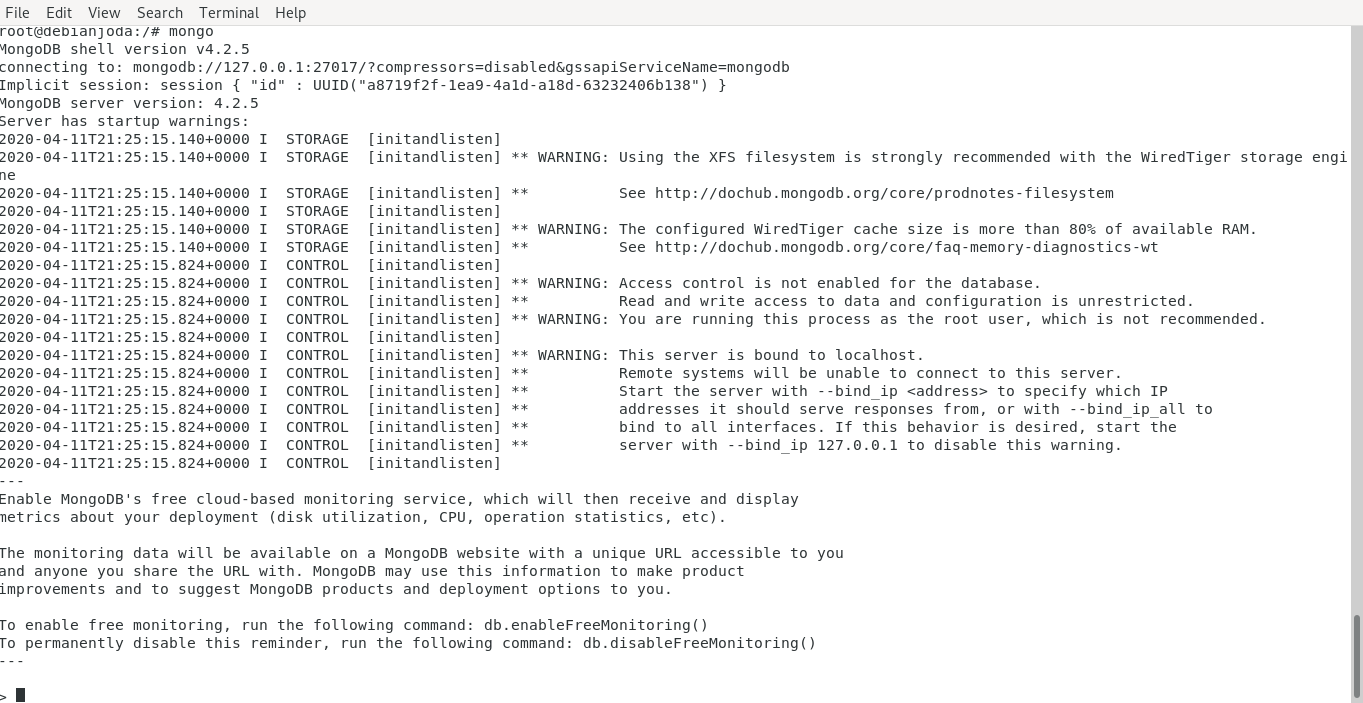
\includegraphics[width=\linewidth]{images/mongoRunning.png}
\caption{Mongo proces pokrenut}
\end{figure}
Bilo bi poželjno mongoDB pokrenuti povezujući je sa drugom IP adresom jer je po prvobitnim postavkama povezana na localhost tj. 127.0.0.1 te može primati zahtjeve samo od aplikacija koje su na toj mašini na kojoj je instaliran mongo. Ovaj korak nije dio ovog praktičnog rada.
\begin{lstlisting}[style=BashInputStyle]
Start the server with --bind_ip <address> to specify which IP addresses it should serve responses from, or with --bind_ip_all to bind to all interfaces.
\end{lstlisting}
\noindent
Nakon završetka instalacije je izvršeno unutar chroot "čišćenje":
\begin{lstlisting}[style=BashInputStyle]
apt-get clean
rm -rf /tmp/* ~/.bash_history
rm -rf /tmp/* ~/.bashrc
rm /var/lib/dbus/machine-id
rm /sbin/initctl
dpkg-divert --rename --remove /sbin/initctl
umount /proc || umount -lf /proc
umount /sys
umount /dev/pts
umount /dev
exit
\end{lstlisting}

\noindent
Generisanje filesystem.manifest datoteke je urađeno u odnosu na edit-mongodb direktorij:
\begin{lstlisting}[style=BashInputStyle]
sudo chmod +w extract-mongodb-cd/casper/filesystem.manifest
sudo su
chroot edit-mongodb dpkg-query -W --showformat='${Package} ${Version}\n' > extract-mongodb-cd/casper/filesystem.manifest
exit
sudo cp extract-mongodb-cd/casper/filesystem.manifest extract-mongodb-cd/casper/filesystem.manifest-desktop
sudo sed -i '/ubiquity/d' extract-mongodb-cd/casper/filesystem.manifest-desktop
sudo sed -i '/casper/d' extract-mongodb-cd/casper/filesystem.manifest-desktop
\end{lstlisting}

\subsection*{Generisanje filesystem.squashfs datoteke - MongoDB modul}
\addcontentsline{toc}{subsection}{\numberline{}Generisanje filesystem.squashfs datoteke - MongoDB modul}
\noindent
Pomoću funkcije iz squashfs-tools, mksquashfs, je kompresovan edit-mongodb direktorij u novu filesystem.squashfs datoteku. U kodu ispod su navedene 3 primjera mksquashfs funkcije. Za kompresiju filesytem.squashfs datoteke odabran je drugi primjer mksquashfs komande:
\begin{lstlisting}[style=BashInputStyle]
sudo rm extract-mongodb-cd/casper/filesystem.squashfs
sudo mksquashfs edit-mongodb extract-mongodb-cd/casper/filesystem.squashfs -nolzma 
sudo mksquashfs edit-mongodb extract-mongodb-cd/casper/filesystem.squashfs -b 1048576
sudo mksquashfs edit-mongodb extract-mongodb-cd/casper/filesystem.squashfs -comp xz -e edit-mongodb/boot
\end{lstlisting}

\noindent
U ovom slučaju filesystem.size datoteka je ažurirana naspram edit-mongodb direktorija:
\begin{lstlisting}[style=BashInputStyle]
sudo su
printf $(du -sx --block-size=1 edit-mongodb | cut -f1) > extract-mongodb-cd/casper/filesystem.size
exit
\end{lstlisting}

\noindent
Prije pozivanja genisoimage funkcijem, upisan je naziv unutar README.diskdefines, 'Ubuntu with MONGODB 18.04.4 LTS "Bionic Beaver" - Release amd64' u polje DISKNAME:
\begin{lstlisting}[style=BashInputStyle]
sudo gedit extract-mongodb-cd/README.diskdefines
\end{lstlisting}

\subsection*{Generisanje Ubuntu .iso image sa mongoDB modulom}
\addcontentsline{toc}{subsection}{\numberline{}Generisanje Ubuntu .iso image sa mongoDB modulom}
\noindent
Ažuriranje md5sum.txt datoteke unutar extract-mongodb-cd direktorija:
\begin{lstlisting}[style=BashInputStyle]
cd extract-mongodb-cd
sudo rm md5sum.txt
find -type f -print0 | sudo xargs -0 md5sum | grep -v isolinux/boot.cat | sudo tee md5sum.txt
\end{lstlisting}

\noindent
Upotrebom funkcije genisoimage, kreirana je .iso datoteka koja sadrži MongoDB modul. Neke Linux distribucije nude mkisofs funkciju. Tako da ukoliko ne radi genisoimage funkcija, ta distribucija bi trebala da podržava funkciju mkisofs:
\begin{lstlisting}[style=BashInputStyle]
sudo genisoimage -D -r -V "$IMAGE_NAME" -cache-inodes -J -l -b isolinux/isolinux.bin -c isolinux/boot.cat -no-emul-boot -boot-load-size 4 -boot-info-table -o ../ubuntu-with-mongodb-18.04-amd64.iso .
\end{lstlisting}

\subsection*{Pokretanje iso datoteke pomoću KVM biblioteke}
\addcontentsline{toc}{subsection}{\numberline{}Pokretanje iso datoteke pomoću KVM biblioteke}
\indent
Kao i za modul NodeJS kreiran je virtuelni tvrdi disk pomoću qemu-img komande da bi se pokrenula datoteka ubuntu-with-mongodb-18.04-amd64.iso.
\begin{lstlisting}[style=BashInputStyle]
cd ~
qemu-img create ubuntumongodb.img 5G
\end{lstlisting}

\noindent 
Pokrenuta je .iso datoteka pomoću KVM-a:
\begin{lstlisting}[style=BashInputStyle]
sudo kvm -hda ubuntumongodb.img -cdrom ~/zavrsni/livecdtmp/ubuntu-with-mongodb-18.04-amd64.iso -boot d -m 2048
\end{lstlisting}

\subsection*{Rezultat Modul MongoDB}
\addcontentsline{toc}{subsection}{\numberline{}Rezultat Modul MongoDB}
\indent
Slika ispod prikazuje MongoDB dostupan unutar Ubuntu distribucije, ubuntu-with-mongodb-18.04-amd64.iso, pokrenutoj sa KVM-om:
\begin{figure}[!htb]
\centering
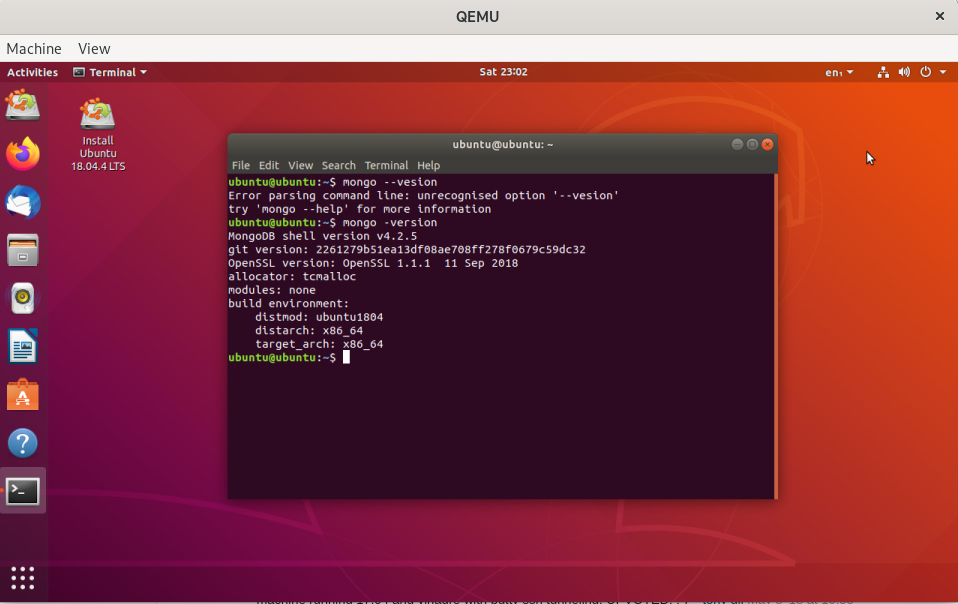
\includegraphics[width=\linewidth]{images/mongoLive.png}
\caption{Mongo proces pokrenut unutar live distribucije}
\end{figure}
\section*{Modul Java}
\addcontentsline{toc}{section}{\numberline{}Modul Java}
Java je objektno-orijentisani programski jezik opće namjene. Aplikacije napisane u Java programskom jeziku se prije izvršenja kompajliraju u Java bitkod te se izvršavaju u Java virtuelnoj mašini, tako da jedan java program može da se pokrene na bilo kom računaru koji ima instaliran Java Virtual Machine.\\
Java je napravljena od strane Sun Microsystems kompanije te objavljena u maju 1995. godine. Posljednja verzija Java-e je 14, dok je posljednja LTS verzija 11. Postoji nekoliko različitih platformi za koje se distribuira Java, te iz toga se mogu definisati 4 grupe Java distribucija:\\
\indent
1. Java Card - za kartice\\
\indent
2. Java Platform, Micro Edition (ME) - za računare sa ograničenim resursima\\
\indent
3. Java Platform, Standard Edition (SE) - za takozvane radne stanice ili "workstations"\\
\indent
4. Java Platform, Enterprise Edition (EE) - za velike distribuirane poslovne sisteme i internet okruženja\\
\indent
Slijedi postupak kreiranja Java modula.

\subsection*{Kreiranje direktorija potrebnih za rad - Java modul}
\addcontentsline{toc}{subsection}{\numberline{}Kreiranje direktorija potrebnih za rad - Java modul}
\indent
Za potrebe kreiranja Java modula kreirani su direktoriji extract-java-cd i edit-java:
\begin{lstlisting}[style=BashInputStyle]
cd ~/squashfs/livecdtmp
sudo mount -o loop ./isoimgs/ubuntu-18.04.4-desktop-amd64.iso mnt
mkdir extract-java-cd
sudo rsync --exclude=/casper/filesystem.squashfs -a mnt/ extract-java-cd
\end{lstlisting}

\subsection*{unsquashfs filesystem.squashs datoteke - Java modul}
\addcontentsline{toc}{subsection}{\numberline{}unsquashfs filesystem.squashfs datoteke - Java modul}
\indent
Raspakovan je ponovo filesystem.squashfs direktorij i kopiran u edit-java direktorij. Razlika ovaj put je ta da je edit direktorij za ovaj modul, imenovan edit-java da ne bi  prethodni sadržaj edit direktorija bio izgubljen, koji je iskorišten za NodeJS modul.\\
\begin{lstlisting}[style=BashInputStyle]
sudo unsquashfs mnt/casper/filesystem.squashfs
sudo mv squashfs-root/ edit-java
\end{lstlisting}
Na slici ispod se vidi ispis unsquashfs komande:
\begin{figure}[!htb]
\centering
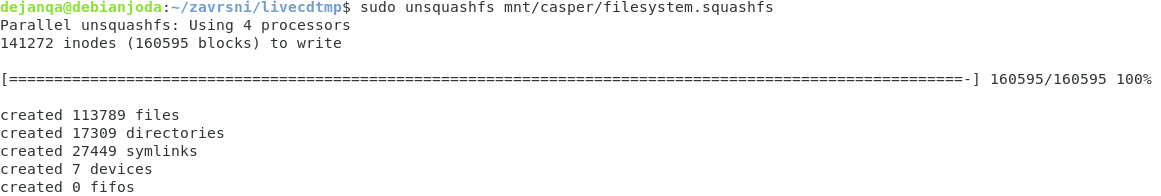
\includegraphics[width=\linewidth]{images/unsquashfscommand.png}
\caption{Ispis unsquashfs komande}
\end{figure}
\subsection*{Konfiguracija paketa za chroot okruženje - Java modul}
\addcontentsline{toc}{subsection}{\numberline{}Konfiguracija paketa za chroot okruženje - Java modul}
\noindent
Ažuriranje resolv.conf unutar edit-java direktorija:
\begin{lstlisting}[style=BashInputStyle]
sudo gedit edit-java/etc/resolv.conf
\end{lstlisting}
Uneseni sadržaj u resolv.conf datoteku:\\
(\textit{nameserver 1.1.1.1 \\
nameserver 8.8.8.8}).\\
\noindent
Ažuriranje etc/hosts datoteke:
\begin{lstlisting}[style=BashInputStyle]
sudo gedit edit-java/etc/hosts
\end{lstlisting}
Uneseni sadržaj u edit-java/etc/hosts datoteku:
\begin{lstlisting}
127.0.0.1	localhost
127.0.1.1	debianjoda.joda.net	debianjoda
\end{lstlisting}

\noindent
Urađena je konfiguracija /dev direktorija kao i za prethodne module. Zatim pokrenuto chroot okruženje u edit-java direktoriju:
\begin{lstlisting}[style=BashInputStyle]
sudo mount --bind /dev/ edit-java/dev
sudo chroot edit-java
mount -t proc none /proc
mount -t sysfs none /sys
mount -t devpts none /dev/pts
\end{lstlisting}

\noindent
Konfiguracija sistemskih varijabli:
\begin{lstlisting}[style=BashInputStyle]
export HOME=/root
export LC_ALL=C
\end{lstlisting}

\subsection*{Instalacija Java paketa unutar chroot okruženja}
\addcontentsline{toc}{subsection}{\numberline{}Instalacija Java paketa unutar chroot okruženja}
\noindent
Za ispis svih instaliranih paketa unutar chroot okruženja:
\begin{lstlisting}[style=BashInputStyle]
dpkg-query -W --showformat='\${Installed-Size}\t\${Package}\n' | sort -nr | less
\end{lstlisting}

\noindent
Instalacija java paketa\cite{apt-java-ubuntu-install}\cite{java-ubuntu-install}
\begin{lstlisting}[style=BashInputStyle]
apt update
apt install default-jdk
\end{lstlisting}
Provjera verzije java instalacije:
\begin{lstlisting}[style=BashInputStyle]
java -version
\end{lstlisting}
Potvrda uspješno instaliranih java paketa:
\begin{lstlisting}[style=BashInputStyle]
openjdk version "11.0.6" 2020-01-14
OpenJDK Runtime Environment (build 11.0.6+10-post-Ubuntu-1ubuntu118.04.1)
OpenJDK 64-Bit Server VM (build 11.0.6+10-post-Ubuntu-1ubuntu118.04.1, mixed mode, sharing)
\end{lstlisting}
Kao praktična primjena Java platforme, instaliran je Eclipse, koji je jedan od najpoznatijih JAVA IDE (Integrated Development Environment)\cite{eclipse-ubuntu-install}
\begin{lstlisting}[style=BashInputStyle]
wget http://ftp.jaist.ac.jp/pub/eclipse/technology/epp/downloads/release/2019-03/R/eclipse-java-2019-03-R-linux-gtk-x86_64.tar.gz
tar -zxvf eclipse-java-2019-03-R-linux-gtk-x86_64.tar.gz -C /usr/
ln -s /usr/eclipse/eclipse /usr/bin/eclipse
nano /usr/share/applications/eclipse.desktop
\end{lstlisting}
Ažurirani sadržaj eclipse.desktop datoteke:
\begin{lstlisting}[style=BashInputStyle]
[Desktop Entry]
Encoding=UTF-8
Name=Eclipse IDE
Comment=Eclipse IDE
Exec=/usr/bin/eclipse
Icon=/usr/eclipse/icon.xpm
Terminal=false
Type=Application
StartupNotify=false
\end{lstlisting}
Eclipse će kasnije biti pokrenut u odjejlku 'Pokretanje .iso datoteke pomoću kvm biblioteke'.
\noindent
Nakon završetka instalacije Java i Eclipse programa, izvršeno je čišćenje unutar chroot okruženja:
\begin{lstlisting}[style=BashInputStyle]
apt clean
rm -rf /tmp/* ~/.bash_history
rm -rf /tmp/* ~/.bashrc
rm /var/lib/dbus/machine-id
rm /sbin/initctl
dpkg-divert --rename --remove /sbin/initctl
umount /proc || umount -lf /proc
umount /sys
umount /dev/pts
umount /dev
exit
\end{lstlisting}

\noindent
Datoteka filesystem.manifest je ažurirana na osnovu edit-java direktorija:
\begin{lstlisting}[style=BashInputStyle]
sudo chmod +w extract-java-cd/casper/filesystem.manifest
sudo su
chroot edit-java dpkg-query -W --showformat='${Package} ${Version}\n' > extract-java-cd/casper/filesystem.manifest
exit
sudo cp extract-java-cd/casper/filesystem.manifest extract-java-cd/casper/filesystem.manifest-desktop
sudo sed -i '/ubiquity/d' extract-java-cd/casper/filesystem.manifest-desktop
sudo sed -i '/casper/d' extract-java-cd/casper/filesystem.manifest-desktop
\end{lstlisting}

\subsection*{Generisanje filesystem.squashfs datoteke - Java modul}
\addcontentsline{toc}{subsection}{\numberline{}Generisanje filesystem.squashfs datoteke - Java modul}
\noindent
Sa funkcijom mksquashfs je kompresovan edit-java direktorij u novu filesystem.squashfs datoteku, baš kao i u prethodna dva slučaja sa MongoDB i NodeJS modulima. Iz isječka koda prikazanog ispod, izvršene su komande iz linije 1 i linije 3:
\begin{lstlisting}[style=BashInputStyle]
sudo rm extract-java-cd/casper/filesystem.squashfs
sudo mksquashfs edit-java extract-java-cd/casper/filesystem.squashfs -nolzma 
sudo mksquashfs edit-java extract-java-cd/casper/filesystem.squashfs -b 1048576
sudo mksquashfs edit-java extract-java-cd/casper/filesystem.squashfs -comp xz -e edit/boot
\end{lstlisting}

\noindent
Datoteka filesystem.size je ažurirana na osnovu edit-java direktorija:
\begin{lstlisting}[style=BashInputStyle]
sudo su
printf $(du -sx --block-size=1 edit-java | cut -f1) > extract-java-cd/casper/filesystem.size
exit
\end{lstlisting}

\noindent
Također upisan je naziv unutar README.diskdefines, 'Ubuntu with Java 18.04.4 LTS "Bionic Beaver" - Release amd64' u polje DISKNAME:
\begin{lstlisting}[style=BashInputStyle]
sudo gedit extract-java-cd/README.diskdefines
\end{lstlisting}

\subsection*{Generisanje Ubuntu .iso image sa Java modulom}
\addcontentsline{toc}{subsection}{\numberline{}Generisanje Ubuntu .iso image sa Java modulom}
\noindent
Ažuriranje md5sum.txt datoteke unutar extract-java-cd direktorija:
\begin{lstlisting}[style=BashInputStyle]
cd extract-java-cd
sudo rm md5sum.txt
find -type f -print0 | sudo xargs -0 md5sum | grep -v isolinux/boot.cat | sudo tee md5sum.txt
\end{lstlisting}

\noindent
Funkcijom genisoimage je kreirana datoteka ubuntu-with-java-18.04-amd64.iso:
\begin{lstlisting}[style=BashInputStyle]
sudo genisoimage -D -r -V "$IMAGE_NAME" -cache-inodes -J -l -b isolinux/isolinux.bin -c isolinux/boot.cat -no-emul-boot -boot-load-size 4 -boot-info-table -o ../ubuntu-with-java-18.04-amd64.iso .
\end{lstlisting}

\subsection*{Pokretanje iso datoteke pomoću KVM biblioteke}
\addcontentsline{toc}{subsection}{\numberline{}Pokretanje iso datoteke pomoću KVM biblioteke}
\indent
Kreiranje virtuelnog tvrdog disk pomoću qemu-img komande u kojem će biti pokrenut modul Java Ubuntu.
\begin{lstlisting}[style=BashInputStyle]
cd ~
qemu-img create ubuntujava.img 5G
\end{lstlisting}

\noindent 
Pomoću KVM-a, pokrenut je ubuntu-with-java-18.04-amd64.iso:
\begin{lstlisting}[style=BashInputStyle]
sudo kvm -hda ubuntujava.img -cdrom ~/zavrsni/livecdtmp/ubuntu-with-java-18.04-amd64.iso -boot d -m 2048
\end{lstlisting}

\subsection*{Rezultat Modul Java}
\addcontentsline{toc}{subsection}{\numberline{}Rezultat Modul Java}
\indent
Modul Java je instaliran u ubuntu-with-java-18.04-amd64.iso.
Slike ispod prikazuju verziju Jave i Eclipse okruženje pokrenuto unutar KVM:
\begin{figure}[!htb]
\centering
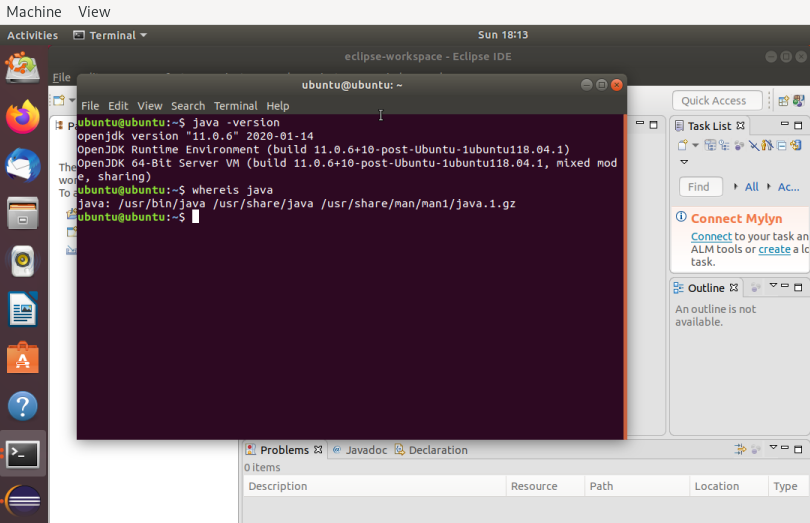
\includegraphics[width=\linewidth]{images/javaLive.png}
\caption{Java verzija u live distribuciji}
\end{figure}
\begin{figure}[!htb]
\centering
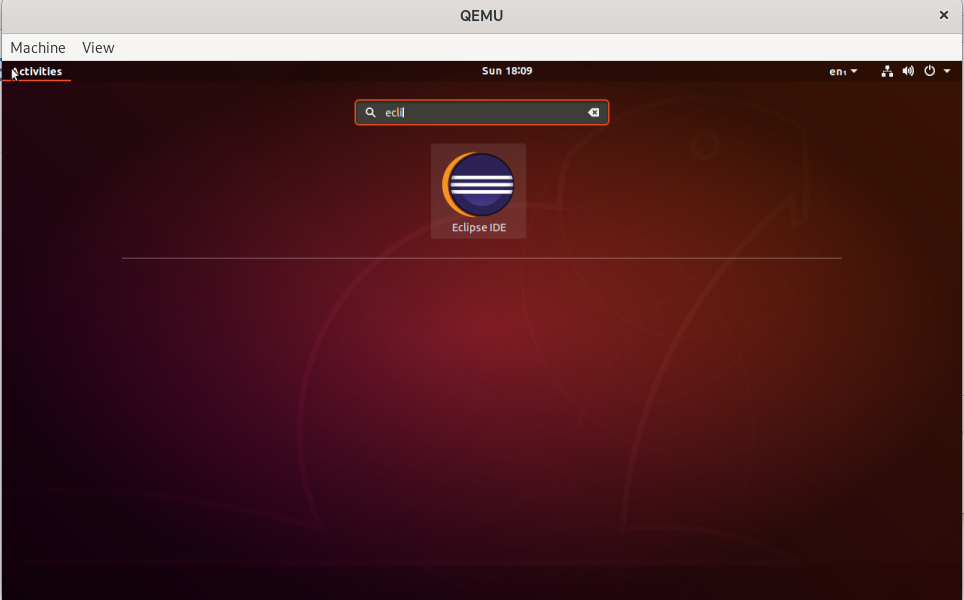
\includegraphics[width=\linewidth]{images/eclipseLive.png}
\caption{Eclipse okruženje u live distribuciji}
\end{figure}
\begin{figure}[!htb]
\centering
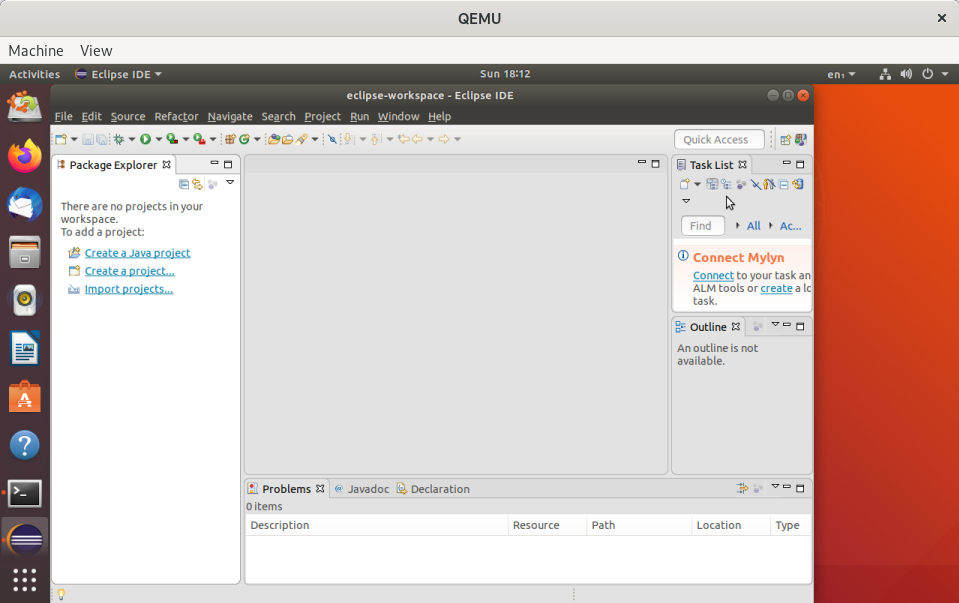
\includegraphics[width=\linewidth]{images/eclipseLive1.png}
\caption{Eclipse okruženje u live distribuciji}
\end{figure}
\newpage
\section*{Modul Chrome}
\addcontentsline{toc}{section}{\numberline{}Modul Chrome}
\indent
Kao četvrti primjer modifikacije squashfs datotečnog sistema, kreiran je modul Chrome. Kao što mu ime kaže, riječ je o modulu sa instaliranim Google Chrome pretraživačem. Većinom koraci su slični kao kod kreiranja prethodnih modula, izuzev koraka instaliranja dodatnih paketa unutar chroot okruženja, i određenih nazivnih konvencija.\\
\indent
Google Chrome je mrežni pretraživač razvijen 2008. godine, prvo za Microsoft Windows, a kasnije i za Linux, MacOS, Android, iOS. Danas, 68\% od ukupnog broja pretraživača na desktop računarima su Google Chrome pretraživači. Sličan je procenat i kada su u pitanju mobilni uređaji.\\
\indent
Google Chrome je najpoznatiji web pretraživač vjerovatno zbog svoje brzine i jednostavnosti za povezivanje različitih uređaja putem Google korisničkog računa. Na većini Android uređaja Google Chrome dođe kao predinstaliran program. Glavne zasluge za dobre performanse Google Chrome pretraživača nosi Google V8 JavaScript virtuelna mašina, koju također koristi i NodeJS.
\subsection*{Kreiranje direktorija potrebnih za rad - Chrome modul}
\addcontentsline{toc}{subsection}{\numberline{}Kreiranje direktorija potrebnih za rad - Chrome modul}
\indent
Za modul Google Chrome su kreirani direktoriji edit-chrome i extract-chrome-cd:
\begin{lstlisting}[style=BashInputStyle]
cd ~/squashfs/livecdtmp
sudo mount -o loop ./isoimgs/ubuntu-18.04.4-desktop-amd64.iso mnt
mkdir extract-chrome-cd
sudo rsync --exclude=/casper/filesystem.squashfs -a mnt/ extract-chrome-cd
\end{lstlisting}

\subsection*{unsquashfs filesystem.squashs datoteke - Chrome modul}
\addcontentsline{toc}{subsection}{\numberline{}unsquashfs filesystem.squashfs datoteke}
\indent
Datoteka filesystem.squashfs je raspakovana i iskopirana u edit-chrome direktorij:\\
\begin{lstlisting}[style=BashInputStyle]
sudo unsquashfs mnt/casper/filesystem.squashfs
sudo mv squashfs-root/ edit-chrome
\end{lstlisting}

\subsection*{Konfiguracija paketa za chroot okruženje - Chrome modul}
\addcontentsline{toc}{subsection}{\numberline{}Konfiguracija paketa za chroot okruženje - Chrome modul}
\indent
Ažuriranje resolv.conf datoteke u edit-chrome direktoriju:
\begin{lstlisting}[style=BashInputStyle]
sudo gedit edit-chrome/etc/resolv.conf
\end{lstlisting}
Ažurirani sadržaj resolv.conf datoteke:\\
\textit{nameserver 1.1.1.1 \\
nameserver 8.8.8.8}\\
\noindent
Ažuriranje etc/hosts datoteke:
\begin{lstlisting}[style=BashInputStyle]
sudo gedit edit-chrome/etc/hosts
\end{lstlisting}
Ažurirani sadržaj etc/hosts datoteke:
\begin{lstlisting}
127.0.0.1	localhost
127.0.1.1	debianjoda.joda.net	debianjoda
\end{lstlisting}

\noindent
Potrebne konfiguracije za chroot okruženje edit-chrome direktorija:
\begin{lstlisting}[style=BashInputStyle]
sudo mount --bind /dev/ edit-chrome/dev
sudo chroot edit-chrome
mount -t proc none /proc
mount -t sysfs none /sys
mount -t devpts none /dev/pts
\end{lstlisting}
\noindent
Konfiguracija sistemskih varijabli:
\begin{lstlisting}[style=BashInputStyle]
export HOME=/root
export LC_ALL=C
\end{lstlisting}

\subsection*{Instalacija Google Chrome paketa unutar chroot okruženja}
\addcontentsline{toc}{subsection}{\numberline{}Instalacija Google Chrome paketa unutar chroot okruženja}
\noindent
Za ispis svih instaliranih paketa:
\begin{lstlisting}[style=BashInputStyle]
dpkg-query -W --showformat='\${Installed-Size}\t\${Package}\n' | sort -nr | less
\end{lstlisting}

\noindent
Ažuriranje google-chrome.list datoteke:
\begin{lstlisting}[style=BashInputStyle]
sudo nano /etc/apt/sources.list.d/google-chrome.list
\end{lstlisting}
Ažurirani sadržaj google-chrome.list datoteke:
\begin{lstlisting}[style=BashInputStyle]
deb [arch=amd64] http://dl.google.com/linux/chrome/deb/ stable main
\end{lstlisting}
\begin{figure}[!htb]
\centering
\includegraphics[width=\linewidth]{images/google-chorme-list.png}
\caption{google-chrme-list datoteka}
\end{figure}
\noindent
Preuzimanje Google javnog ključa je potrebno za instaliranje Google Chrome paketa. Također potrebno je komandom apt-key dodati ključ u prsten javnih ključeva da bi apt mogao potvrditi integritet Google Chrome paketa.\\
\begin{lstlisting}[style=BashInputStyle]
wget https://dl.google.com/linux/linux_signing_key.pub
sudo apt-key add linux_signing_key.pub
\end{lstlisting}
\noindent
Izlaz prethodne komande je "OK" u slučaju da nije došlo do greške.\\
\indent
Ažuriranje liste paketa i instaliranje google-chrome-stable paketa:
\begin{lstlisting}[style=BashInputStyle]
apt update
apt install google-chrome-stable
\end{lstlisting}
\noindent
Provjera instalacije:
\begin{lstlisting}[style=BashInputStyle]
google-chrome-stable --version
\end{lstlisting}
\begin{figure}[!htb]
\centering
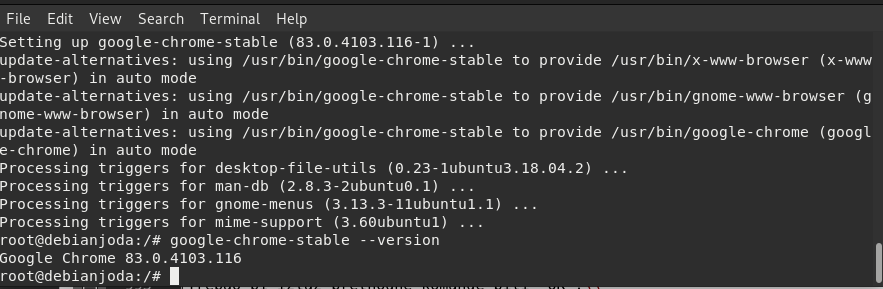
\includegraphics[width=\linewidth]{images/googlechromestableversion.png}
\caption{Google Chrome verzija}
\end{figure}
\noindent
Nakon završetka instalacije urađeno je čišćenje unutar chroot:
\begin{lstlisting}[style=BashInputStyle]
apt clean
rm -rf /tmp/* ~/.bash_history
rm -rf /tmp/* ~/.bashrc
rm /var/lib/dbus/machine-id
rm /sbin/initctl
dpkg-divert --rename --remove /sbin/initctl
umount /proc || umount -lf /proc
umount /sys
umount /dev/pts
umount /dev
exit
\end{lstlisting}

\noindent
Datoteka filesystem.manifest je ažurirana na osnovu edit-chrome direktorija:
\begin{lstlisting}[style=BashInputStyle]
sudo chmod +w extract-chrome-cd/casper/filesystem.manifest
sudo su
chroot edit-chrome dpkg-query -W --showformat='${Package} ${Version}\n' > extract-chrome-cd/casper/filesystem.manifest
exit
sudo cp extract-chrome-cd/casper/filesystem.manifest extract-chrome-cd/casper/filesystem.manifest-desktop
sudo sed -i '/ubiquity/d' extract-chrome-cd/casper/filesystem.manifest-desktop
sudo sed -i '/casper/d' extract-chrome-cd/casper/filesystem.manifest-desktop
\end{lstlisting}

\subsection*{Generisanje filesystem.squashfs datoteke - Chrome modul}
\addcontentsline{toc}{subsection}{\numberline{}Generisanje filesystem.squashfs datoteke - Chrome modul}
\noindent
Iz paketa squashfs-tools, mksquashfs funkcijom je kompresovan edit-chrome direktorij u novu filesystem.squashfs datoteku. U kodu ispod je izvršena komanda iz linije 1 komanda na liniji 3:
\begin{lstlisting}[style=BashInputStyle]
sudo rm extract-chrome-cd/casper/filesystem.squashfs
sudo mksquashfs edit-chrome extract-chrome-cd/casper/filesystem.squashfs -nolzma 
sudo mksquashfs edit-chrome extract-chrome-cd/casper/filesystem.squashfs -b 1048576
sudo mksquashfs edit-chrome extract-chrome-cd/casper/filesystem.squashfs -comp xz -e edit/boot
\end{lstlisting}

\noindent
Ažuriranje filesystem.size datoteke:
\begin{lstlisting}[style=BashInputStyle]
sudo su
printf $(du -sx --block-size=1 edit-chrome | cut -f1) > extract-chrome-cd/casper/filesystem.size
exit
\end{lstlisting}

\noindent
Upisan je naziv unutar README.diskdefines, 'Ubuntu with Google Chrome 18.04.4 LTS "Bionic Beaver" - Release amd64' u polje DISKNAME:
\begin{lstlisting}[style=BashInputStyle]
sudo gedit extract-chrome-cd/README.diskdefines
\end{lstlisting}

\subsection*{Generisanje Ubuntu .iso image sa Google Chrome modulom}
\addcontentsline{toc}{subsection}{\numberline{}Generisanje Ubuntu .iso image sa Google Chrome modulom}
\noindent
Prije pokretanja .iso datoteke sa instaliranim Google Chrome modulom ažurirana md5sum.txt datoteka:
\begin{lstlisting}[style=BashInputStyle]
cd extract-chrome-cd
sudo rm md5sum.txt
find -type f -print0 | sudo xargs -0 md5sum | grep -v isolinux/boot.cat | sudo tee md5sum.txt
\end{lstlisting}

\noindent
Funkcijom genisoimage kreirana je ubuntu-with-chrome-18.04-amd64.iso datoteka koja sadrži Google Chrome modul:
\begin{lstlisting}[style=BashInputStyle]
sudo genisoimage -D -r -V "$IMAGE_NAME" -cache-inodes -J -l -b isolinux/isolinux.bin -c isolinux/boot.cat -no-emul-boot -boot-load-size 4 -boot-info-table -o ../ubuntu-with-chrome-18.04-amd64.iso .
\end{lstlisting}

\subsection*{Pokretanje iso image-a pomoću kvm biblioteke}
\addcontentsline{toc}{subsection}{\numberline{}Pokretanje iso image-a pomoću kvm biblioteke}
\indent
I za ovaj modul kreiran je virtuelni tvrdi disk pomoću qemu-img komande:
\begin{lstlisting}[style=BashInputStyle]
cd ~
qemu-img create ubuntuchrome.img 5G
\end{lstlisting}

\noindent 
Modul Google Chrome je pokrenut pomoću KVM-a:
\begin{lstlisting}[style=BashInputStyle]
sudo kvm -hda ubuntuchrome.img -cdrom ~/zavrsni/livecdtmp/ubuntu-with-chrome-18.04-amd64.iso -boot d -m 2048
\end{lstlisting}

\subsection*{Rezultat Modul Chrome}
\addcontentsline{toc}{subsection}{\numberline{}Rezultat Modul Chrome}
\indent
Nakon pokretanja ubuntu-with-chrome-18.04-amd64.iso u KVM, odabirom opcije Try Ubuntu možemo se uvjeriti da je Google Chrome instaliran, što pokazuju slike ispod:
\begin{figure}[!htb]
\centering
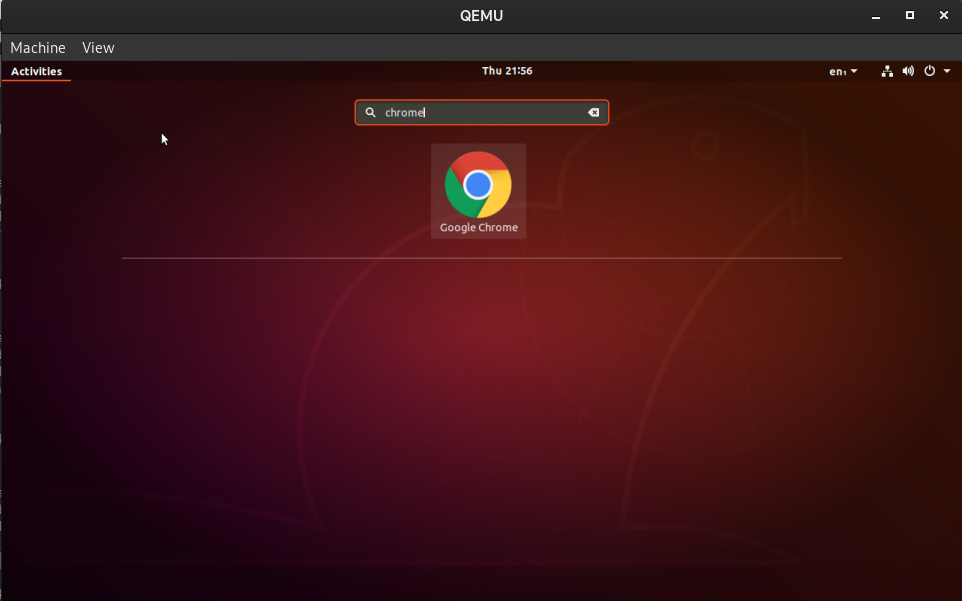
\includegraphics[width=\linewidth]{images/chromeLive.png}
\caption{Google Chrome u live distribuciji}
\end{figure}
\begin{figure}[!htb]
\centering
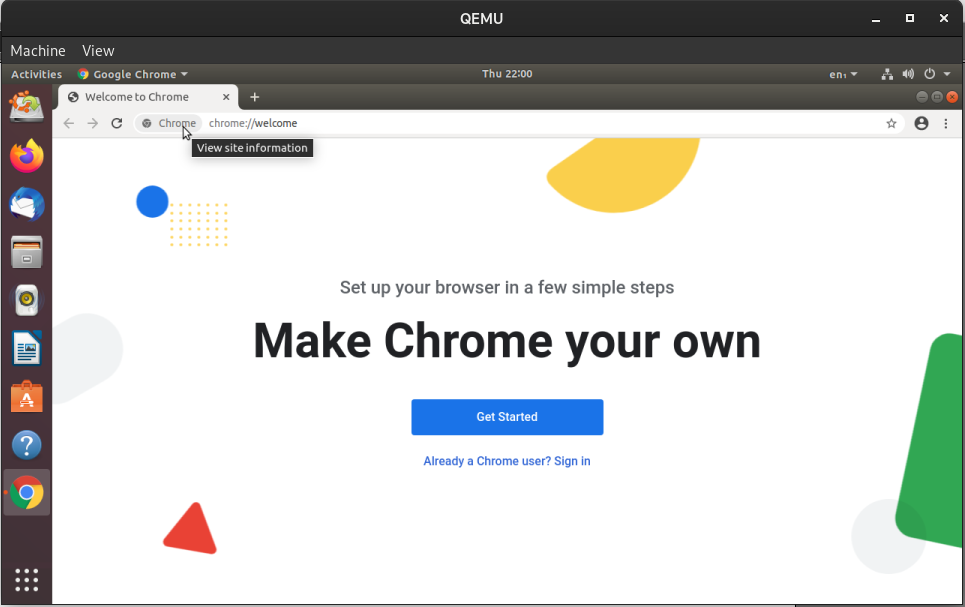
\includegraphics[width=\linewidth]{images/chromeLive2.png}
\caption{Google Chrome u live distribuciji}
\end{figure}
\chapter*{Kreiranje više modula unutar jedne .iso datoteke}
\addcontentsline{toc}{chapter}{\numberline{}Kreiranje više modula unutar jedne .iso datoteke}
\indent
U prethodnom dijelu rada je opisan proces kreiranja zasebnih .iso datoteka za svaki od modula. U nastavku rada je opisan proces kreiranja jedne modularne .iso datoteke u kojoj će biti sadržani svi moduli koji su prethodno pojedinačno kreirani.\\
Ovakav pristup podrazumijeva više filesystem.squashfs datoteka unutar jedne .iso datoteke. Cilj je da se kreira jedan bazni modul koji sadrži baznu filesystem.squashfs datoteku i ostale *.squashfs datoteke od pojedinih modula. Ova bazna filesystem.squashfs datoteka je jedina kompletna squashfs datoteka. Ostale squasfhfs datoteke sadrže razlike između datotečnih sistema pojedinih modula sa baznim datotečnim sistemom.\\
Delta funkcije su izvršene naspram edit direktorija a sve *.squashfs datoteke se naposljetku smještaju u bazni-modul direktorij.
\indent
Razlika izmedju edit direktorija pojedinih modula sa baznim edit direktorijem su datoteke instaliranih paketa, kao što su java paketi, nodejs paketi, google-chrome paketi i mongodb paketi. Pored ovih razlika postoji i jedna bitna datoteka koja će se razlikovati, a to je /var/lib/dpkg/status datoteka. Ona sadrži popis svih instaliranih paketa. Za svaki modul je napravljen delta direktorij koji sadrži razlike između baznog edit direktorija sa edit direktorijem pojedinog modula. Također unutar delta direktorija je kreirana status.diff datoteku koja sadrži razliku status datoteke baznog edit direktorija i status datoteke edit direktorija pojedinog modula.\\
\indent
Deaktivacija pojedinog modula bi podrazumijeva izvršavanje umount komande tog modula, koja se može izvršiti dok je sistem pokrenut. Također podrazumijeva i ponovno generisanje status datoteke pri čemu je nova status datoteka razlika između bazne status datoteke i status.diff datoteke tog modula. Ovaj koncept aktivacije i deaktivacije je izvan opsega ovog rada, te je spomenut samo kao moguće unaprijeđenje.

\section*{Bazni modul}
\addcontentsline{toc}{section}{\numberline{}Bazni modul}
\indent
Direktorij bazni-modul je odredišni direktorij koji sadrži sve .squashfs datoteke. Od njega se naposljetku generiše .iso datoteka koja sadrži sve module, za razliku od pristupa opisanog u prethodnom poglavlju gdje su generisane 4 zasebne iso datoteke, za svaki modul po jedna.\\
Kao početna stavka ovog dijela rada kreiran je bazni-modul direktorij koji je raspakovana ubuntu-18.04.4-desktop-amd64.iso datoteka sa izmjenama u etc/hosts i etc/resolv.conf datotekama. Izmjene u ove dvije datoteke su neophodne da unutar KVM-a pri pokretanju .iso datoteke radi mrežna konekcija.\\
Montiranje ubuntu-18.04.4-desktop-amd64.iso datoteku na mnt direktorij:
\begin{lstlisting}[style=BashInputStyle]
sudo mount -o loop ./isoimgs/ubuntu-18.04.4-desktop-amd64.iso mnt
\end{lstlisting}

Konfiguracija direktorija pod nazivom bazni-modul u u kojeg je kopiran mnt direktorij izostavljajući filesystem.squashfs datoteku unutar /casper direktorija:
\begin{lstlisting}[style=BashInputStyle]
mkdir bazni-modul
sudo rsync --exclude=/casper/filesystem.squashfs -a mnt/ bazni-modul
\end{lstlisting}
Kasnije u nastavku će biti generisane .squashfs datoteke koje će biti pozicionirane u /casper direktorij bazni-modul direktorija.

\section*{Bazni edit}
\addcontentsline{toc}{section}{\numberline{}Bazni edit}
\indent
Koristeći unsquashfs funkciju raspakovana je kompresovana filesystem.squashfs datoteku te sadržaj kopiran u direktorij pod nazivom bazni-edit. Unutar ovog direktorija su podešene opće mrežne postavke u hosts i resolv.conf datotekama.
\begin{lstlisting}[style=BashInputStyle]
sudo unsquashfs mnt/casper/filesystem.squashfs
sudo mv squashfs-root/ bazni-edit
\end{lstlisting}

Ažuriranje resolv.conf datoteke u bazni-edit/etc direktoriju:
\begin{lstlisting}[style=BashInputStyle]
sudo gedit bazni-edit/etc/resolv.conf
\end{lstlisting}
\noindent
Sadržaj ažurirane resolv.conf\cite{wiki-resolv.conf} datoteke:\\
(\textit{nameserver 1.1.1.1 \\
nameserver 8.8.8.8}).\\
\noindent
Ažuriranje etc/hosts\cite{wiki-hosts-file} datoteke:
\begin{lstlisting}[style=BashInputStyle]
sudo gedit bazni-edit/etc/hosts
\end{lstlisting}
Ažurirani sadržaj hosts datoteke:
\begin{lstlisting}
127.0.0.1	localhost
127.0.1.1	debianjoda.joda.net	debianjoda
\end{lstlisting}

\noindent
Još nam ostaje podešavanje bazni-edit/dev direktorija. To ćemo postići kao i u prethodnim koracima gdje smo pravili zasebne iso image-e od pojedinih modula, kopirajući /dev/ direktorij sa hosta, zatim chroot u bazni-edit direktorij, te izvršavanje mount instrukcija navedenih ispod:
\begin{lstlisting}[style=BashInputStyle]
sudo mount --bind /dev/ bazni-edit/dev
sudo chroot bazni-edit
mount -t proc none /proc
mount -t sysfs none /sys
mount -t devpts none /dev/pts
\end{lstlisting}

\noindent
Također potrebno je izvršiti sljedeće komande da bi se izbjegli problemi sa lokalizacijom:
\begin{lstlisting}[style=BashInputStyle]
export HOME=/root
export LC_ALL=C
\end{lstlisting}

Potom ćemo izvršiti čišćenje unutar chroot okruženja te komandom exit izaći iz chroot okruženja:
\begin{lstlisting}[style=BashInputStyle]
apt-get clean
rm -rf /tmp/* ~/.bash_history
rm -rf /tmp/* ~/.bashrc
rm /var/lib/dbus/machine-id
rm /sbin/initctl
dpkg-divert --rename --remove /sbin/initctl
umount /proc || umount -lf /proc
umount /sys
umount /dev/pts
umount /dev
exit
\end{lstlisting}
\indent
Konfiguracija bazni-edit direktorija je kompletna. Iz ovog direktorija su napravljeni edit direktoriji ostalih modula. Napomena da se u nastavku procesa također ponavljaju neke komande koje su potrebne za izvršenje, uz razlike u nazivima direktorija i datoteka. Svakako je primjetno da su i u prethodnom dijelu rada također komande više puta ponovljene za iste dijelova procesa za pojedine module, ali je od velike važnosti izvršavanje komandi redoslijedom, stoga komande nisu izostavljene iako se neke ponavljaju.

\section*{NodeJS edit}
\addcontentsline{toc}{section}{\numberline{}NodeJS edit}
\indent
Ovo poglavlje opisuje proces kreiranja nodejs-edit direktorija koji je upotrijebljen za kreiranje nodejsBazniDelta direktorija. Poglavlje o nodejsBazniDelta direktoriju je u opisano u poglavlju 'Generisanje nodejs.squashfs direktorija - Kreiranje nodejsBazniDelta direktorija'.\\
Kreiranje nodejs-edit direktorija:
\begin{lstlisting}[style=BashInputStyle]
mkdir nodejs-edit
sudo rsync -a bazni-edit/ nodejs-edit
\end{lstlisting}
\noindent
Konfiguracija chroot okruženja za nodejs-edit direktorij:
\begin{lstlisting}[style=BashInputStyle]
sudo mount --bind /dev/ nodejs-edit/dev
sudo chroot nodejs-edit
mount -t proc none /proc
mount -t sysfs none /sys
mount -t devpts none /dev/pts
\end{lstlisting}
\noindent
Podešavanje sistemskih varijabli:
\begin{lstlisting}[style=BashInputStyle]
export HOME=/root
export LC_ALL=C
\end{lstlisting}
\noindent
Instalacija nodejs paketa:
\begin{lstlisting}[style=BashInputStyle]
apt-get update
apt-get install curl
curl -sL https://deb.nodesource.com/setup_13.x | sudo -E bash -
apt-get install -y nodejs
\end{lstlisting}
\noindent
Potvrda instalacije nodejs paketa:
\begin{lstlisting}[style=BashInputStyle]
node --version
\end{lstlisting}
\noindent
Nakon završetka instalacije urađeno je čišćenje unutar chroot okruženja za nodejs-edit direktorij:
\begin{lstlisting}[style=BashInputStyle]
apt-get clean
rm -rf /tmp/* ~/.bash_history
rm -rf /tmp/* ~/.bashrc
rm /var/lib/dbus/machine-id
rm /sbin/initctl
dpkg-divert --rename --remove /sbin/initctl
umount /proc || umount -lf /proc
umount /sys
umount /dev/pts
umount /dev
exit
\end{lstlisting}

Konfiguracija nodejs-edit direktorija je dovršena. Direktorij nodejs-edit je upotrijebljenj za poređenje sa bazni-edit direktorijem za dobijanje delta direktorija između 2 direktorija. Od delta direktorija je kreirana nodejs.squashfs datoteka. Datoteka nodejs.squashfs će biti kopirana u bazni-modul/casper direktorij.

\section*{MongoDB edit}
\addcontentsline{toc}{section}{\numberline{}MongoDB edit}
Ovo poglavlje opisuje proces konfiguracije mongodb-edit direktorija. Direktorij mongodb-edit je iskorišten za generisanje mongodbBaziDelta direktorija, iz kojeg je kreirana mongodb.squashfs datoteka.\\
\noindent
Generisanje mongodb-edit direktorija:
\begin{lstlisting}[style=BashInputStyle]
mkdir mongodb-edit
sudo rsync -a bazni-edit/ mongodb-edit
\end{lstlisting}

\noindent
Konfiguracija mongodb-edit direktorija i priprema za chroot okruženje:
\begin{lstlisting}[style=BashInputStyle]
sudo mount --bind /dev/ mongodb-edit/dev
sudo chroot mongodb-edit
mount -t proc none /proc
mount -t sysfs none /sys
mount -t devpts none /dev/pts
\end{lstlisting}
\noindent
Podešavanje sistemskih varijabli:
\begin{lstlisting}[style=BashInputStyle]
export HOME=/root
export LC_ALL=C
\end{lstlisting}

\noindent
Instaliranje libcurl4 i openssl paketa, neophodnih za pokretanje MongoDB servisa:
\begin{lstlisting}[style=BashInputStyle]
apt-get update
apt-get install libcurl4 openssl
\end{lstlisting}
\noindent
Preuzimanje MongoDB paketa sa interneta:
\begin{lstlisting}[style=BashInputStyle]
wget https://fastdl.mongodb.org/linux/mongodb-linux-x86_64-ubuntu1804-4.2.5.tgz
\end{lstlisting}
\noindent
Ekstrakcija paketa:
\begin{lstlisting}[style=BashInputStyle]
tar -zxvf mongodb-linux-x86_64-ubuntu1804-4.2.5.tgz
\end{lstlisting}
\noindent
Kopiranje mongodb bin direktorij u /usr/local/bin/ direktorij:
\begin{lstlisting}[style=BashInputStyle]
cp mongodb-linux-x86_64-ubuntu1804-4.2.5/bin/* /usr/local/bin/
\end{lstlisting}
\noindent
Konfiguracija mongo direktorija za podatke:
\begin{lstlisting}[style=BashInputStyle]
mkdir -p /var/lib/mongo
\end{lstlisting}
\noindent
Konfiguracija mongodb direktorija za logove:
\begin{lstlisting}[style=BashInputStyle]
mkdir -p /var/log/mongodb
\end{lstlisting}
\noindent
Ažuriranje privilegija pristupa na mongo i mongodb direktorije:
\begin{lstlisting}[style=BashInputStyle]
chown `whoami` /var/lib/mongo 
chown `whoami` /var/log/mongodb
\end{lstlisting}
\noindent
Pokretanje mongod proces:
\begin{lstlisting}[style=BashInputStyle]
mongod --dbpath /var/lib/mongo --logpath /var/log/mongodb/mongod.log --fork
\end{lstlisting}
\noindent
Provjera instalacije:
\begin{lstlisting}[style=BashInputStyle]
mongo --version
\end{lstlisting}
\noindent
Ispis komande nakon uspješno instaliranog mongodb paketa:
\begin{lstlisting}[style=BashInputStyle]
MongoDB shell version v4.2.5
git version: 2261279b51ea13df08ae708ff278f0679c59dc32
OpenSSL version: OpenSSL 1.1.1  11 Sep 2018
allocator: tcmalloc
modules: none
build environment:
    distmod: ubuntu1804
    distarch: x86_64
    target_arch: x86_64
\end{lstlisting}
\noindent
Nakon završetka instalacije urađeno je unutar chroot "čišćenje":
\begin{lstlisting}[style=BashInputStyle]
apt-get clean
rm -rf /tmp/* ~/.bash_history
rm -rf /tmp/* ~/.bashrc
rm /var/lib/dbus/machine-id
rm /sbin/initctl
dpkg-divert --rename --remove /sbin/initctl
umount /proc || umount -lf /proc
umount /sys
umount /dev/pts
umount /dev
exit
\end{lstlisting}

Opisan je proces kreiranja mongodb-edit direktorija. On će biti upotrijebljen za poređenje sa bazni-edit direktorijem. Od tog delta direktorija će biti stvorena mongodb.squashfs datoteka.

\section*{Java edit}
\addcontentsline{toc}{section}{\numberline{}Java edit}
\indent
Ovo poglavlje opisuje proces konfiguracije java-edit direktorija, kasnije iskorištenog za generisanje javaBazniDelta direktorija, na osnovu kojeg je kreiran java.squashfs modul.\\
\noindent
Generisanje java-edit direktorija:
\begin{lstlisting}[style=BashInputStyle]
mkdir java-edit
sudo rsync -a bazni-edit/ java-edit
\end{lstlisting}
\noindent
Konfiguracija i podešavanje za chroot okruženje java-edit direktorija:
\begin{lstlisting}[style=BashInputStyle]
sudo mount --bind /dev/ java-edit/dev
sudo chroot java-edit
mount -t proc none /proc
mount -t sysfs none /sys
mount -t devpts none /dev/pts
\end{lstlisting}
\noindent
Podešavanje sistemskih varijabli:
\begin{lstlisting}[style=BashInputStyle]
export HOME=/root
export LC_ALL=C
\end{lstlisting}
\noindent
Instalacija java paketa:
\begin{lstlisting}[style=BashInputStyle]
apt update
apt install default-jdk
\end{lstlisting}
\noindent
Provjera verzije java instalacije:
\begin{lstlisting}[style=BashInputStyle]
java -version
\end{lstlisting}
\noindent
Rezultat uspješne java instalacije:
\begin{lstlisting}[style=BashInputStyle]
openjdk version "11.0.8" 2020-07-14
OpenJDK Runtime Environment (build 11.0.8+10-post-Ubuntu-0ubuntu118.04.1)
OpenJDK 64-Bit Server VM (build 11.0.8+10-post-Ubuntu-0ubuntu118.04.1, mixed mode, sharing)
\end{lstlisting}
\noindent
Instaliran je Eclipse, koji je već spomenut u prethodnom odjeljku Modul Java:
\begin{lstlisting}[style=BashInputStyle]
wget http://ftp.jaist.ac.jp/pub/eclipse/technology/epp/downloads/release/2019-03/R/eclipse-java-2019-03-R-linux-gtk-x86_64.tar.gz
tar -zxvf eclipse-java-2019-03-R-linux-gtk-x86_64.tar.gz -C /usr/
ln -s /usr/eclipse/eclipse /usr/bin/eclipse
nano /usr/share/applications/eclipse.desktop
\end{lstlisting}
Ažuriranje eclipse.desktop datoteke:
\begin{lstlisting}[style=BashInputStyle]
[Desktop Entry]
Encoding=UTF-8
Name=Eclipse IDE
Comment=Eclipse IDE
Exec=/usr/bin/eclipse
Icon=/usr/eclipse/icon.xpm
Terminal=false
Type=Application
StartupNotify=false
\end{lstlisting}

\noindent
Čišćenje unutar chroot okruženja nakon instalacije:
\begin{lstlisting}[style=BashInputStyle]
apt clean
rm -rf /tmp/* ~/.bash_history
rm -rf /tmp/* ~/.bashrc
rm /var/lib/dbus/machine-id
rm /sbin/initctl
dpkg-divert --rename --remove /sbin/initctl
umount /proc || umount -lf /proc
umount /sys
umount /dev/pts
umount /dev
exit
\end{lstlisting}
Kompletiran je proces konfiguracije java-edit direktorija. Ovaj edit direktorij će biti upoređen sa bazni-edit direktorijem radi generisanja javaBazniDelta direktorija.
Te će od delte biti pravljen java.squashfs modul.
\section*{Chrome edit}
\addcontentsline{toc}{section}{\numberline{}Chrome edit}
\indent
Ovo poglavlje opisuje konfiguraciju chrome-edit direktorija, u kasnijem poglavlju upotrijebljenog za generisanje chromeBazniDelta direktorija.\\ 
\noindent
Generisanje chrome-edit direktorija:
\begin{lstlisting}[style=BashInputStyle]
mkdir chrome-edit
sudo rsync -a bazni-edit/ chrome-edit
\end{lstlisting}
\noindent
Konfiguracija chroot okruženja za chrome-edit direktorij:
\begin{lstlisting}[style=BashInputStyle]
sudo mount --bind /dev/ chrome-edit/dev
sudo chroot chrome-edit
mount -t proc none /proc
mount -t sysfs none /sys
mount -t devpts none /dev/pts
\end{lstlisting}
\noindent
Podešavanje sistemskih varijabli:
\begin{lstlisting}[style=BashInputStyle]
export HOME=/root
export LC_ALL=C
\end{lstlisting}
\noindent
Ažuriranje google-chrome.list datoteke:
\begin{lstlisting}[style=BashInputStyle]
sudo nano /etc/apt/sources.list.d/google-chrome.list
\end{lstlisting}
\noindent
Ažurirani sadržaj google-chrome.list datoteke:
\begin{lstlisting}[style=BashInputStyle]
deb [arch=amd64] http://dl.google.com/linux/chrome/deb/ stable main
\end{lstlisting}
\begin{figure}[!htb]
\centering
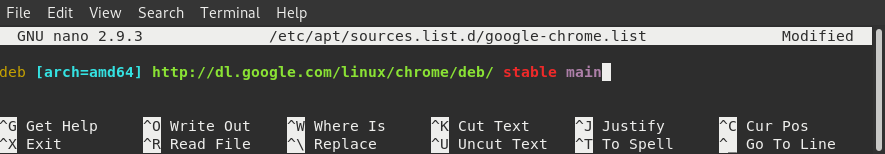
\includegraphics[width=\linewidth]{images/google-chrome-list.png}
\caption{google-chrome-list}
\end{figure}
\noindent
Sljedeća komanda preuzima Google javni ključ. Komanda apt-key dodaje ključ u prsten javnih ključeva da bi apt mogao potvrditi integritet Google Chrome paketa:\\
\begin{lstlisting}[style=BashInputStyle]
wget https://dl.google.com/linux/linux_signing_key.pub
sudo apt-key add linux_signing_key.pub
\end{lstlisting}
\noindent
Uspješan ispis prethodne komande treba biti "OK".\\
\noindent
Instalacija google-chrome-stable paketa:
\begin{lstlisting}[style=BashInputStyle]
apt update
apt install google-chrome-stable
\end{lstlisting}
\noindent
Provjera instalacije:
\begin{lstlisting}[style=BashInputStyle]
google-chrome-stable --version
\end{lstlisting}
\begin{figure}[!htb]
\centering
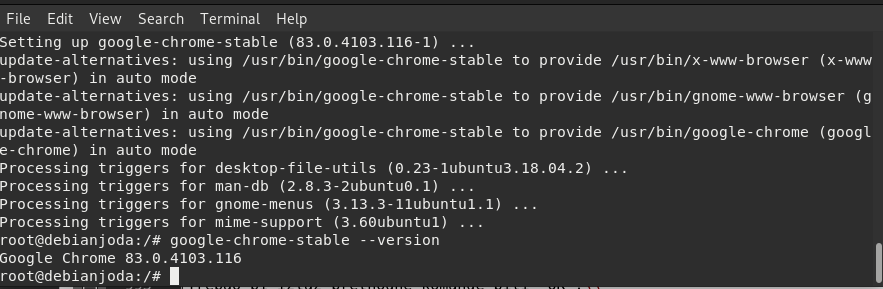
\includegraphics[width=\linewidth]{images/googlechromestableversion.png}
\caption{google-chrome-stable verzija}
\end{figure}
\noindent
Čišćenje unutar chroot okruženja chrome-edit direktorija:
\begin{lstlisting}[style=BashInputStyle]
apt clean
rm -rf /tmp/* ~/.bash_history
rm -rf /tmp/* ~/.bashrc
rm /var/lib/dbus/machine-id
rm /sbin/initctl
dpkg-divert --rename --remove /sbin/initctl
umount /proc || umount -lf /proc
umount /sys
umount /dev/pts
umount /dev
exit
\end{lstlisting}
\indent
Opisan je proces konfiguracije chrome-edit direktorij. On je, kao i prethodni edit direktoriji, iskorišten za poredeđenje sa bazni-edit direktorijem, da bismo dobili delta direktorij. Od delta direktorija je kreirana chrome.squashfs datoteka pozicionirana u bazni-modul/casper direktoriju kao i ostale .squashfs datoteke.

\section*{Generisanje bazne filesystem.squashfs modula}
\addcontentsline{toc}{section}{\numberline{}Generisanje bazne filesystem.squashfs modula}
\indent
Ovo poglavlje opisuje proces generisanje baznog filesystem.squash modula. Direktorij, na osnovu kojeg je kreirana bazna filesystem.squashfs datoteka, je bazni-edit direktorij.\\
\noindent
Ažuriranje bazne filesystem.manifest datoteke:
\begin{lstlisting}[style=BashInputStyle]
sudo chmod +w bazni-modul/casper/filesystem.manifest
sudo su
chroot bazni-edit dpkg-query -W --showformat='${Package} ${Version}\n' > bazni-modul/casper/filesystem.manifest
exit
sudo cp bazni-modul/casper/filesystem.manifest bazni-modul/casper/filesystem.manifest-desktop
sudo sed -i '/ubiquity/d' bazni-modul/casper/filesystem.manifest-desktop
sudo sed -i '/casper/d' bazni-modul/casper/filesystem.manifest-desktop
\end{lstlisting}
\noindent
Generisanje bazne filesystem.squashfs datoteke:
\begin{lstlisting}[style=BashInputStyle]
sudo rm bazni-modul/casper/filesystem.squashfs
sudo mksquashfs bazni-edit bazni-modul/casper/filesystem.squashfs -b 1048576
\end{lstlisting}
\noindent
Ažuriranje filesystem.size datoteke na osnovu bazni-edit direktorija:
\begin{lstlisting}[style=BashInputStyle]
sudo su
printf $(du -sx --block-size=1 bazni-edit | cut -f1) > bazni-modul/casper/filesystem.size
exit
\end{lstlisting}
\noindent
Generisana je bazna filesystem.squashfs datoteka, tj bazni squashfs modul. U nastavku je opisan proces pravljenja ostalih squashfs modula.
\section*{Generisanje nodejs.squashfs modula}
\addcontentsline{toc}{section}{\numberline{}Generisanje nodejs.squashfs modula}
\indent
Proces kreiranja nodejs.squashfs modula podrazumijeva prije svega generisanje delta direktorija koji sadrži sve razlike između bazni-edit i nodejs-edit direktorija. Također se podrazumijeva kreiranje status.diff datoteke koja će sadržati razliku između status datoteka bazni-edit i nodejs-edit direktorija.
\subsection*{Kreiranje nodejsBazniDelta direktorija}
\addcontentsline{toc}{subsection}{\numberline{}Kreiranje nodejsBazniDelta direktorija}
\indent
Od nodejsBazniDelta direktorija će biti kreiran modul nodejs.squashfs.\\
Iskorištena je komanda rsync sa atributima -rvclm:\\
-r = --recursive - rekurzivna pretraga po direktorijima\\
-v = --verbose - detaljniji ispis informacija tokom izvršenja komande\\
-c = --checksum - ne kopirati samo ako su checksum-i jednaki\\
-l = --links - kopirati symbolic links\\
-m = --prune-empty-dirs - ne kopirati prazne direktorije\\
\begin{lstlisting}[style=BashInputStyle]
mkdir nodejsBazniDelta
sudo rsync -rvclm --compare-dest=/home/user/zavrsni/livecdtmp/bazni-edit/ /home/user/zavrsni/livecdtmp/nodejs-edit/ /home/user/zavrsni/livecdtmp/nodejsBazniDelta/
\end{lstlisting}
\indent
U nodejsBazniDelta direktorij je presmještena i status.diff datoteka koja sadrži razliku između status datoteka bazni-edit i nodejs-edit direktorija. To je postignuto diff komandom:
\begin{lstlisting}[style=BashInputStyle]
sudo diff bazni-edit/var/lib/dpkg/status nodejs-edit/var/lib/dpkg/status > status.diff
\end{lstlisting}
Sadržaj diff datoteke je izmijenjen u smislu da je obrisan početni karatker svakog reda koji je generisan od diff komande a to je karakter '>'.\\
U ovom konkretnom slučaju sadržaj status.diff datoteke je sljedeći:
\begin{lstlisting}[style=BashInputStyle]
Package: curl
Status: install ok installed
Priority: optional
Section: web
Installed-Size: 387
Maintainer: Ubuntu Developers <ubuntu-devel-discuss@lists.ubuntu.com>
Architecture: amd64
Multi-Arch: foreign
Version: 7.58.0-2ubuntu3.10
Depends: libc6 (>= 2.17), libcurl4 (= 7.58.0-2ubuntu3.10), zlib1g (>= 1:1.1.4)
Description: command line tool for transferring data with URL syntax
 curl is a command line tool for transferring data with URL syntax, supporting
 DICT, FILE, FTP, FTPS, GOPHER, HTTP, HTTPS, IMAP, IMAPS, LDAP, LDAPS, POP3,
 POP3S, RTMP, RTSP, SCP, SFTP, SMTP, SMTPS, TELNET and TFTP.
 .
 curl supports SSL certificates, HTTP POST, HTTP PUT, FTP uploading, HTTP form
 based upload, proxies, cookies, user+password authentication (Basic, Digest,
 NTLM, Negotiate, kerberos...), file transfer resume, proxy tunneling and a
 busload of other useful tricks.
Homepage: http://curl.haxx.se
Original-Maintainer: Alessandro Ghedini <ghedo@debian.org>

Package: nodejs
Status: install ok installed
Priority: optional
Section: web
Installed-Size: 114614
Maintainer: Chris Lea <chl@nodesource.com>
Architecture: amd64
Version: 13.14.0-1nodesource1
Replaces: nodejs-dev (<= 0.8.22), nodejs-legacy, npm (<= 1.2.14)
Provides: nodejs-dev, nodejs-legacy, npm
Depends: libc6 (>= 2.17), libgcc1 (>= 1:3.4), libstdc++6 (>= 4.8), python-minimal, ca-certificates
Conflicts: nodejs-dev, nodejs-legacy, npm
Description: Node.js event-based server-side javascript engine
 Node.js is similar in design to and influenced by systems like
 Ruby's Event Machine or Python's Twisted.
 .
 It takes the event model a bit further - it presents the event
 loop as a language construct instead of as a library.
 .
 Node.js is bundled with several useful libraries to handle server tasks :
 System, Events, Standard I/O, Modules, Timers, Child Processes, POSIX,
 HTTP, Multipart Parsing, TCP, DNS, Assert, Path, URL, Query Strings.
Homepage: https://nodejs.org

Package: libcurl4
Status: install ok installed
Priority: optional
Section: libs
Installed-Size: 627
Maintainer: Ubuntu Developers <ubuntu-devel-discuss@lists.ubuntu.com>
Architecture: amd64
Multi-Arch: same
Source: curl
Version: 7.58.0-2ubuntu3.10
Replaces: libcurl3
Depends: libc6 (>= 2.17), libgssapi-krb5-2 (>= 1.14+dfsg), libidn2-0 (>= 0.6), libldap-2.4-2 (>= 2.4.7), libnghttp2-14 (>= 1.12.0), libpsl5 (>= 0.13.0), librtmp1 (>= 2.4+20131018.git79459a2-3~), libssl1.1 (>= 1.1.1), zlib1g (>= 1:1.1.4)
Recommends: ca-certificates
Conflicts: libcurl3
Description: easy-to-use client-side URL transfer library (OpenSSL flavour)
 libcurl is an easy-to-use client-side URL transfer library, supporting DICT,
 FILE, FTP, FTPS, GOPHER, HTTP, HTTPS, IMAP, IMAPS, LDAP, LDAPS, POP3, POP3S,
 RTMP, RTSP, SCP, SFTP, SMTP, SMTPS, TELNET and TFTP.
 .
 libcurl supports SSL certificates, HTTP POST, HTTP PUT, FTP uploading, HTTP
 form based upload, proxies, cookies, user+password authentication (Basic,
 Digest, NTLM, Negotiate, Kerberos), file transfer resume, http proxy tunneling
 and more!
 .
 libcurl is free, thread-safe, IPv6 compatible, feature rich, well supported,
 fast, thoroughly documented and is already used by many known, big and
 successful companies and numerous applications.
 .
 SSL support is provided by OpenSSL.
Homepage: http://curl.haxx.se
Original-Maintainer: Alessandro Ghedini <ghedo@debian.org>
\end{lstlisting}
\indent
Premještanje status.diff datoteke u nodejsBazniDelta/var/lib/dpkg direktorij:
\begin{lstlisting}[style=BashInputStyle]
sudo rm nodejsBazniDelta/var/lib/dpkg/status
sudo mv status.diff nodejsBazniDelta/var/lib/dpkg/status
\end{lstlisting}

\subsection*{nodejs.squashfs datoteka}
\addcontentsline{toc}{subsection}{\numberline{}nodejs.squashfs datoteka}
\indent
Generisanje nodejs.manifest datoteke, slične baznoj filesystem.manifest datoteci, prethodi generisanju nodejs.squashfs datoteke:
\begin{lstlisting}[style=BashInputStyle]
sudo su
chroot nodejs-edit dpkg-query -W --showformat='${Package} ${Version}\n' > bazni-modul/casper/nodejs.manifest
exit
sudo cp bazni-modul/casper/nodejs.manifest bazni-modul/casper/nodejs.manifest-desktop
sudo sed -i '/ubiquity/d' bazni-modul/casper/nodejs.manifest-desktop
sudo sed -i '/casper/d' bazni-modul/casper/nodejs.manifest-desktop
\end{lstlisting}
\indent
Generisanje nodejs.squashfs modula na osnovu nodejsBazniDelta direktorija:
\begin{lstlisting}[style=BashInputStyle]
sudo mksquashfs nodejsBazniDelta bazni-modul/casper/nodejs.squashfs -b 1048576
\end{lstlisting}
\noindent
Ažuriranje nodejs.size datoteke na osnovu nodejsBazniDelta direktorija:
\begin{lstlisting}[style=BashInputStyle]
sudo su
printf $(du -sx --block-size=1 nodejsBazniDelta | cut -f1) > bazni-modul/casper/nodejs.size
exit
\end{lstlisting}
Završen je proces za kreiranje nodejs.squashfs datoteke. Kao i bazna filesystem.squashfs datoteka, i nodejs.squashfs datoteka je smještena u bazni-modul/casper direktorij.
\section*{Generisanje mongodb.squashfs modula}
\addcontentsline{toc}{section}{\numberline{}Generisanje mongodb.squashfs modula}
\indent
U ovom je dijelu opisan proces kreiranja mongodb.squashfs modula. Proces kreiranja mongodb.squashfs datoteke zahtijeva prije svega generisanje delta direktorija koji sadrži sve razlike između bazni-edit i mongodb-edit direktorija. Također se podrazumijeva kreiranje status.diff datoteke koja sadrži razliku između status datoteka bazni-edit i mongodb-edit direktorija.\\

\subsection*{Kreiranje mongodbBazniDelta direktorija}
\addcontentsline{toc}{subsection}{\numberline{}Kreiranje mongodbBazniDelta direktorija}
\indent
Ovaj dio opisuje proces kreiranja mongodbBazniDelta direktorija.
Kao i u slučaju nodejsBazniDelta direktorije, korištena je komanda rsync sa atributima -rvclm:\\
\noindent
-r = --recursive - rekurzivna pretraga po direktorijima\\
\noindent
-v = --verbose - detaljniji ispis informacija tokom izvršenja komande\\
\noindent
-c = --checksum - ne kopirati samo ako su checksum-i jednaki\\
\noindent
-l = --links - kopirati symbolic links\\
\noindent
-m = --prune-empty-dirs - ne kopirati prazne direktorije\\
\begin{lstlisting}[style=BashInputStyle]
mkdir mongodbBazniDelta
sudo rsync -rvclm --compare-dest=/home/user/zavrsni/livecdtmp/bazni-edit/ /home/user/zavrsni/livecdtmp/mongodb-edit/ /home/user/zavrsni/livecdtmp/mongodbBazniDelta/
\end{lstlisting}
\noindent
U mongodbBazniDelta direktorij je također ubačena status.diff datoteka koja sadrži razliku između status datoteka bazni-edit i mongodb-edit direktorija. Pomoću diff komande je generisanje status.diff datoteka:
\begin{lstlisting}[style=BashInputStyle]
sudo diff bazni-edit/var/lib/dpkg/status mongodb-edit/var/lib/dpkg/status > status.diff
\end{lstlisting}
\noindent
Nakon uklanjanja neželjenih karaktera, status.diff datoteka ima sljedeći sadržaj:
\begin{lstlisting}[style=BashInputStyle]
Package: libcurl4
Status: install ok installed
Priority: optional
Section: libs
Installed-Size: 627
Maintainer: Ubuntu Developers <ubuntu-devel-discuss@lists.ubuntu.com>
Architecture: amd64
Multi-Arch: same
Source: curl
Version: 7.58.0-2ubuntu3.10
Replaces: libcurl3
Depends: libc6 (>= 2.17), libgssapi-krb5-2 (>= 1.14+dfsg), libidn2-0 (>= 0.6), libldap-2.4-2 (>= 2.4.7), libnghttp2-14 (>= 1.12.0), libpsl5 (>= 0.13.0), librtmp1 (>= 2.4+20131018.git79459a2-3~), libssl1.1 (>= 1.1.1), zlib1g (>= 1:1.1.4)
Recommends: ca-certificates
Conflicts: libcurl3
Description: easy-to-use client-side URL transfer library (OpenSSL flavour)
 libcurl is an easy-to-use client-side URL transfer library, supporting DICT,
 FILE, FTP, FTPS, GOPHER, HTTP, HTTPS, IMAP, IMAPS, LDAP, LDAPS, POP3, POP3S,
 RTMP, RTSP, SCP, SFTP, SMTP, SMTPS, TELNET and TFTP.
 .
 libcurl supports SSL certificates, HTTP POST, HTTP PUT, FTP uploading, HTTP
 form based upload, proxies, cookies, user+password authentication (Basic,
 Digest, NTLM, Negotiate, Kerberos), file transfer resume, http proxy tunneling
 and more!
 .
 libcurl is free, thread-safe, IPv6 compatible, feature rich, well supported,
 fast, thoroughly documented and is already used by many known, big and
 successful companies and numerous applications.
 .
 SSL support is provided by OpenSSL.
Homepage: http://curl.haxx.se
Original-Maintainer: Alessandro Ghedini <ghedo@debian.org>
\end{lstlisting}
\noindent
Premještanje status.diff datoteke u mongodbBazniDelta direktorij:
\begin{lstlisting}[style=BashInputStyle]
sudo rm mongodbBazniDelta/var/lib/dpkg/status
sudo mv status.diff mongodbBazniDelta/var/lib/dpkg/status
\end{lstlisting}
U narednom poglavlju opisana je procedura za pravljenje mongodb.squashfs datoteke.
\subsection*{mongodb.squashfs datoteka}
\addcontentsline{toc}{subsection}{\numberline{}mongodb.squashfs datoteka}
\indent
Modul mongodb.squashfs se generiše na osnovu mongodbBazniDelta direktorija. Generisan je mongodb.manifest, slično kao kod generisanja nodejs.manifest datoteke samo uz razliku što sad umjesto nodejs je upotrijebljen mongodb prefix:
\begin{lstlisting}[style=BashInputStyle]
sudo su
chroot mongodb-edit dpkg-query -W --showformat='${Package} ${Version}\n' > bazni-modul/casper/mongodb.manifest
exit
sudo cp bazni-modul/casper/mongodb.manifest bazni-modul/casper/mongodb.manifest-desktop
sudo sed -i '/ubiquity/d' bazni-modul/casper/mongodb.manifest-desktop
sudo sed -i '/casper/d' bazni-modul/casper/mongodb.manifest-desktop
\end{lstlisting}
\noindent
Kreiranje mongodb.squashfs datoteke na osnovu mongodbBazniDelta direktorija:
\begin{lstlisting}[style=BashInputStyle] 
sudo mksquashfs mongodbBazniDelta bazni-modul/casper/mongodb.squashfs -b 1048576
\end{lstlisting}
\noindent
Ažuriranje mongodb.size datoteke:
\begin{lstlisting}[style=BashInputStyle]
sudo su
printf $(du -sx --block-size=1 mongodbBazniDelta | cut -f1) > bazni-modul/casper/mongodb.size
exit
\end{lstlisting}
U narednom poglavlju se opisuje proces kreiranja java.squashfs modula.
\section*{Generisanje java.squashfs modula}
\addcontentsline{toc}{section}{\numberline{}Generisanje java.squashfs modula}
\indent
Proces kreiranja java.squashfs datoteke podrazumijeva prije svega generisanje delta direktorija koji sadrži sve razlike između bazni-edit i java-edit direktorija. Također se podrazumijeva kreiranje status.diff datoteke koja sadrži razliku između status datoteka bazni-edit i java-edit direktorija.\\

\subsection*{Kreiranje javaBazniDelta direktorija}
\addcontentsline{toc}{subsection}{\numberline{}Kreiranje javaBazniDelta direktorija}
\indent
Za kreiranje delta direktorija upotrijebljena je komanda rsync sa atributima -rvclm, kao i u prethodnim primjerima:\\
\noindent
-r = --recursive - rekurzivna pretraga po direktorijima\\
\noindent
-v = --verbose - detaljniji ispis informacija tokom izvršenja komande\\
\noindent
-c = --checksum - ne kopirati samo ako su checksum-i jednaki\\
\noindent
-l = --links - kopirati symbolic links\\
\noindent
-m = --prune-empty-dirs - ne kopirati prazne direktorije
\begin{lstlisting}[style=BashInputStyle]
mkdir javaBazniDelta
sudo rsync -rvclm --compare-dest=/home/user/zavrsni/livecdtmp/bazni-edit/ /home/user/zavrsni/livecdtmp/java-edit/ /home/user/zavrsni/livecdtmp/javaBazniDelta/
\end{lstlisting}
\noindent
Pomoću komande diff je generisana status.diff datoteka:
\begin{lstlisting}[style=BashInputStyle]
sudo diff bazni-edit/var/lib/dpkg/status java-edit/var/lib/dpkg/status > status.diff
\end{lstlisting}
\noindent
Nakon uklanjanja neželjenih karaktera iz status.diff datoteke, ista je prebačena u javaBazniDelta/var/lib/dpkg direktorij:
\begin{lstlisting}[style=BashInputStyle]
sudo rm javaBazniDelta/var/lib/dpkg/status
sudo mv status.diff javaBazniDelta/var/lib/dpkg/status
\end{lstlisting}
Dovršen je proces generisanja javaBazniDelta direktorija. Slijedi opis procedure za kreiranje java.squashfs modula.
\subsection*{java.squashfs datoteka}
\addcontentsline{toc}{subsection}{\numberline{}java.squashfs datoteka}
\noindent
Ovaj odjeljak prikazuje proces generisanja java.squashfs modula na osnovu javaBazniDelta direktorija.
Generisan je prvenstveno java.manifest, slično kao kod generisanja nodejs.manifest i mongodb.manifest datoteka samo uz razliku što je iskorišteno odgovarajuće ime modula java kao prefix ispred .manifest nastavka:
\begin{lstlisting}[style=BashInputStyle]
sudo su
chroot java-edit dpkg-query -W --showformat='${Package} ${Version}\n' > bazni-modul/casper/java.manifest
exit
sudo cp bazni-modul/casper/java.manifest bazni-modul/casper/java.manifest-desktop
sudo sed -i '/ubiquity/d' bazni-modul/casper/java.manifest-desktop
sudo sed -i '/casper/d' bazni-modul/casper/java.manifest-desktop
\end{lstlisting}
\noindent
Generisnje java.squshfs datoteke na osnovu javaBazniDelta direktorija:
\begin{lstlisting}[style=BashInputStyle]
sudo mksquashfs javaBazniDelta bazni-modul/casper/java.squashfs -b 1048576
\end{lstlisting}
\noindent
Ažuriranje java.size datoteke:
\begin{lstlisting}[style=BashInputStyle]
sudo su
printf $(du -sx --block-size=1 javaBazniDelta | cut -f1) > bazni-modul/casper/java.size
exit
\end{lstlisting}
Dovršena je procedura jreiranja java.squashfs modula. Slijedi opis procedure za chrome.squashfs modul.
\section*{Generisanje chrome.squashfs modula}
\addcontentsline{toc}{section}{\numberline{}Generisanje chrome.squashfs modula}
\noindent
Proces kreiranja chrome.squashfs modula zahtijeva generisanje delta direktorija koji sadrži sve razlike između bazni-edit i chrome-edit direktorija. Također se podrazumijeva kreiranje status.diff datoteke koja sadrži razliku između status datoteka bazni-edit chrome-edit direktorija.
\subsection*{Kreiranje chromeBazniDelta direktorija}
\addcontentsline{toc}{subsection}{\numberline{}Kreiranje chromeBazniDelta direktorija}
\indent
Pomoću komande rsync sa atributima -rvclm, kreiran je sadržaj delta direktorija:\\
\noindent
-r = --recursive - rekurzivna pretraga po direktorijima\\
\noindent
-v = --verbose - detaljniji ispis informacija tokom izvršenja komande\\
\noindent
-c = --checksum - ne kopirati samo ako su checksum-i jednaki\\
\noindent
-l = --links - kopirati symbolic links\\
\noindent
-m = --prune-empty-dirs - ne kopirati prazne direktorije\\
\begin{lstlisting}[style=BashInputStyle]
mkdir chromeBazniDelta
sudo rsync -rvclm --compare-dest=/home/user/zavrsni/livecdtmp/bazni-edit/ /home/user/zavrsni/livecdtmp/chrome-edit/ /home/user/zavrsni/livecdtmp/chromeBazniDelta/
\end{lstlisting}
\noindent
Generisanje status.diff datoteke za chromeBazniDelta direktorij:
\begin{lstlisting}[style=BashInputStyle]
sudo diff bazni-edit/var/lib/dpkg/status chrome-edit/var/lib/dpkg/status > status.diff
\end{lstlisting}
\noindent
Nakon uklanjanja neželjenih karaktera, status.diff datoteka ima sljedeći sadržaj:
\begin{lstlisting}[style=BashInputStyle]
Package: google-chrome-stable
Status: install ok installed
Priority: optional
Section: web
Installed-Size: 230929
Maintainer: Chrome Linux Team <chromium-dev@chromium.org>
Architecture: amd64
Version: 85.0.4183.83-1
Provides: www-browser
Depends: ca-certificates, fonts-liberation, libappindicator3-1, libasound2 (>= 1.0.16), libatk-bridge2.0-0 (>= 2.5.3), libatk1.0-0 (>= 2.2.0), libatspi2.0-0 (>= 2.9.90), libc6 (>= 2.16), libcairo2 (>= 1.6.0), libcups2 (>= 1.4.0), libdbus-1-3 (>= 1.5.12), libdrm2 (>= 2.4.38), libexpat1 (>= 2.0.1), libgbm1 (>= 8.1~0), libgcc1 (>= 1:3.0), libgdk-pixbuf2.0-0 (>= 2.22.0), libglib2.0-0 (>= 2.39.4), libgtk-3-0 (>= 3.9.10), libnspr4 (>= 2:4.9-2~), libnss3 (>= 2:3.22), libpango-1.0-0 (>= 1.14.0), libpangocairo-1.0-0 (>= 1.14.0), libx11-6 (>= 2:1.4.99.1), libx11-xcb1, libxcb-dri3-0, libxcb1 (>= 1.6), libxcomposite1 (>= 1:0.3-1), libxcursor1 (>> 1.1.2), libxdamage1 (>= 1:1.1), libxext6, libxfixes3, libxi6 (>= 2:1.2.99.4), libxrandr2, libxrender1, libxtst6, wget, xdg-utils (>= 1.0.2)
Pre-Depends: dpkg (>= 1.14.0)
Recommends: libu2f-udev, libvulkan1
Description: The web browser from Google
 Google Chrome is a browser that combines a minimal design with sophisticated technology to make the web faster, safer, and easier.
\end{lstlisting}
\noindent
Prebacivanje status.diff datoteke u odgovarajući direktorij:
\begin{lstlisting}[style=BashInputStyle]
sudo rm chromeBazniDelta/var/lib/dpkg/status
sudo mv status.diff chromeBazniDelta/var/lib/dpkg/status
\end{lstlisting}

\subsection*{chrome.squashfs datoteka}
\addcontentsline{toc}{subsection}{\numberline{}chrome.squashfs datoteka}
\noindent
Generisana je datoteka chrome.manifest unutar bazni-modul direktorija na osnovu chrome-edit direktorija:
\begin{lstlisting}[style=BashInputStyle]
sudo su
chroot chrome-edit dpkg-query -W --showformat='${Package} ${Version}\n' > bazni-modul/casper/chrome.manifest
exit
sudo cp bazni-modul/casper/chrome.manifest bazni-modul/casper/chrome.manifest-desktop
sudo sed -i '/ubiquity/d' bazni-modul/casper/chrome.manifest-desktop
sudo sed -i '/casper/d' bazni-modul/casper/chrome.manifest-desktop
\end{lstlisting}
\noindent
Pravljenje chrome.squashfs datoteke:
\begin{lstlisting}[style=BashInputStyle]
sudo mksquashfs chromeBazniDelta bazni-modul/casper/chrome.squashfs -b 1048576
\end{lstlisting}
\noindent
Ažuriranje chrome.size datoteke:
\begin{lstlisting}[style=BashInputStyle]
sudo su
printf $(du -sx --block-size=1 chromeBazniDelta | cut -f1) > bazni-modul/casper/chrome.size
exit
\end{lstlisting}

\section*{Generisanje ubuntu-cjmn-18.04-amd64.iso datoteke}
\addcontentsline{toc}{section}{\numberline{}Generisanje ubuntu-cjmn-18.04-amd64.iso datoteke}
\indent
Ovo poglavle opisuje proces generisanja .iso datoteke, kao finalnog proizvoda praktičnog rada. Kreirana je .iso datoteka koja sadrži 5 .squashfs modula. Upotrijebljena je skraćenica cjmn u nazivu .iso datoteke. CJMN predstavlja skraćenicu za termine Chrome, Java, MongoDB i NodeJS zajedno.\\
Upisan naziv unutar README.diskdefines u polje DISKNAME, je 'Ubuntu with Chrome/Java/MongoDB/NodeJS 18.04.4 LTS "Bionic Beaver" - Release amd64':
\begin{lstlisting}[style=BashInputStyle]
sudo gedit bazni-modul/README.diskdefines
\end{lstlisting}
\noindent
Ažuriranje md5sum.txt:
\begin{lstlisting}[style=BashInputStyle]
cd bazni-modul
sudo rm md5sum.txt
find -type f -print0 | sudo xargs -0 md5sum | grep -v isolinux/boot.cat | sudo tee md5sum.txt
\end{lstlisting}
\noindent
Generisanje ubuntu-cjmn-18.04-amd64.iso datoteke:
\begin{lstlisting}[style=BashInputStyle]
sudo genisoimage -D -r -V "$IMAGE_NAME" -cache-inodes -J -l -b isolinux/isolinux.bin -c isolinux/boot.cat -no-emul-boot -boot-load-size 4 -boot-info-table -o ../ubuntu-cjmn-18.04-amd64.iso .
\end{lstlisting}

\subsection*{Pokretanje iso image-a pomoću kvm biblioteke}
\addcontentsline{toc}{subsection}{\numberline{}Pokretanje iso image-a pomoću kvm biblioteke}
\indent
Kreiran je virtuelni tvrdi disk pomoću qemu-img komande za pokretanje ubuntu-cjmn-18.04-amd64.iso. Ovom virtuelnom disku je postavljena veličina od 10G, za razliku od prethodno kreiranih virtuelnih diskova sa veličinom od 5G:
\begin{lstlisting}[style=BashInputStyle]
cd ~
qemu-img create ubuntucjmn.img 10G
\end{lstlisting}

\noindent 
Pomoću KVM-a pokrenut je ubuntu-cjmn-18.04-amd64.iso:
\begin{lstlisting}[style=BashInputStyle]
sudo kvm -hda ubuntucjmn.img -cdrom ~/zavrsni/livecdtmp/ubuntu-cjmn-18.04-amd64.iso -boot d -m 2048
\end{lstlisting}

\subsection*{Rezultat ubuntu-cjmn-18.04-amd64.iso}
\addcontentsline{toc}{subsection}{\numberline{}Rezultat ubuntu-cjmn-18.04-amd64.iso}
\indent
Nakon pokretanja ubuntu-cjmn-18.04-amd64.iso datoteke, i odabira opcije Try Ubuntu, možem se provjeriti da su uspješno instalirani moduli Google Chrome, Java, MongoDB, NodeJS, što pokazuju slike ispod:
\begin{figure}[!htb]
\centering
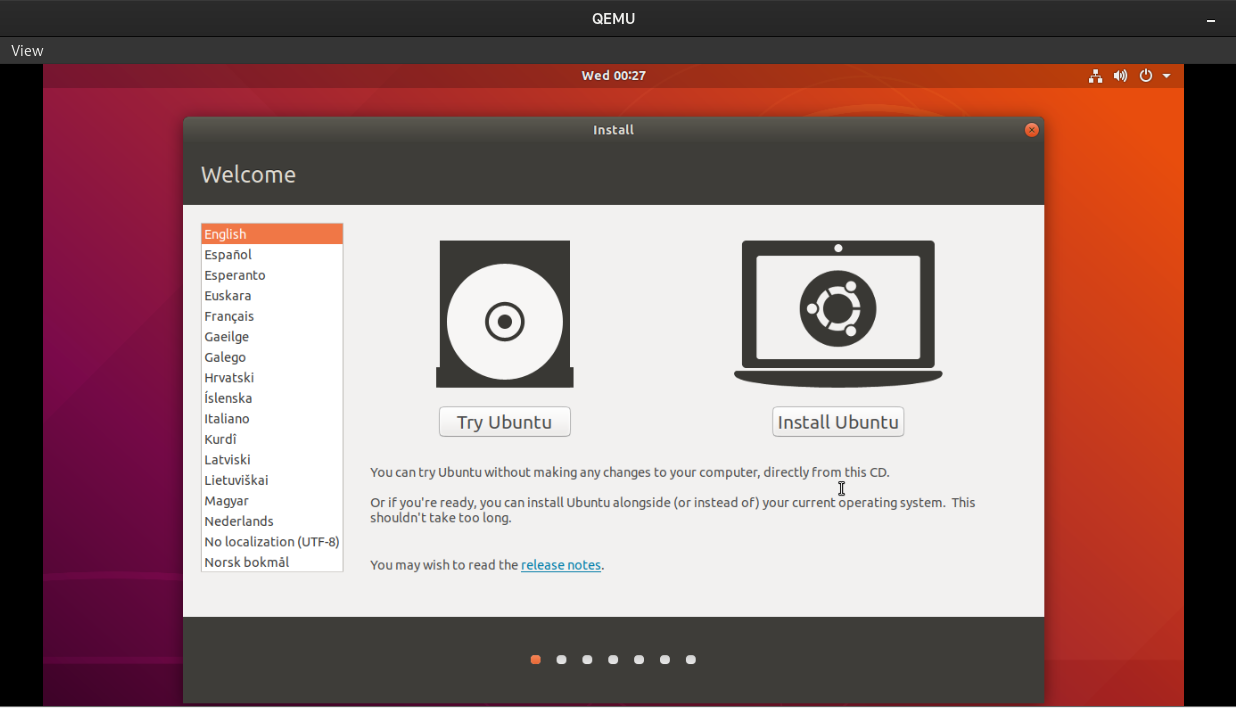
\includegraphics[width=\linewidth]{images/tryUbuntu.png}
\caption{Try Ubuntu}
\end{figure}
\begin{figure}[!htb]
\centering
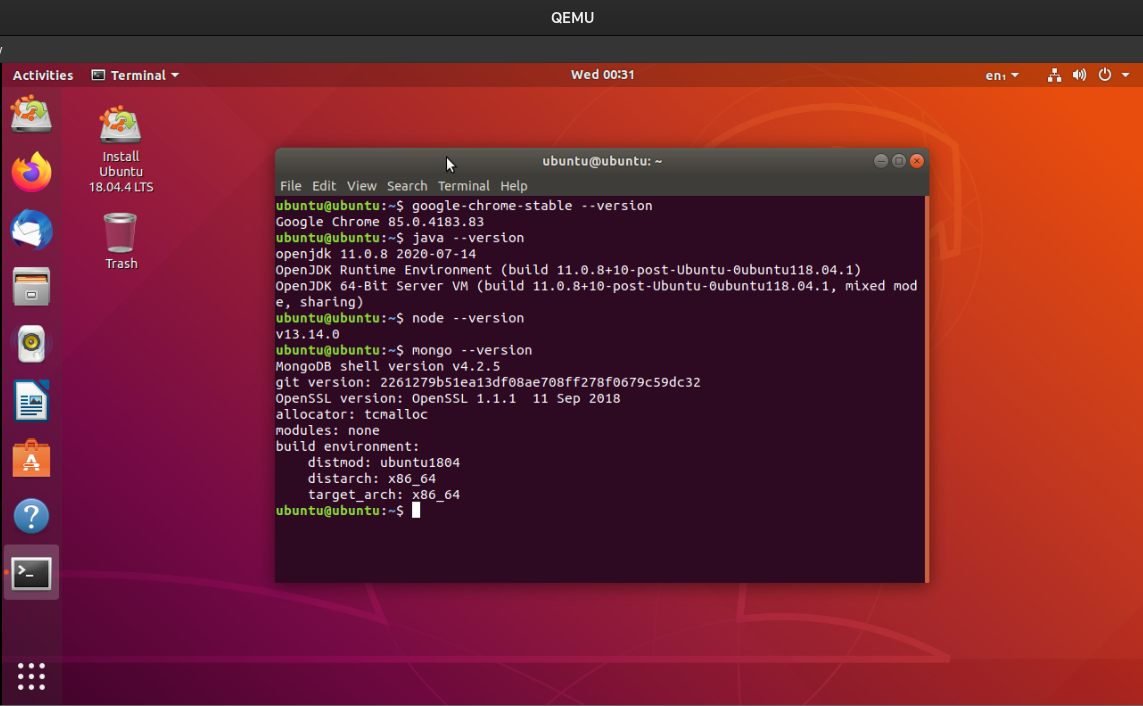
\includegraphics[width=\linewidth]{images/ubuntu-cjmn.png}
\caption{Ubuntu CJMN}
\end{figure}

\chapter*{Zaključak}
\addcontentsline{toc}{chapter}{\numberline{}Zaključak}
\indent
Kao jedan nedostatak rada izdvaja se nedostatak skripte koja izvršava aktivaciju i deaktivaciju modula, koju bi korisnik mogao pozvati u pokrenutoj live distribuciji. Ova skripta bi u pozadini trebala da uključi ili isključi .squashfs datotečni sistem u zavisnosti od modula koji se aktivira ili deaktivira. Pored toga morala bi i status datoteka biti ažurirana gdje bi se sadržaj status.diff datoteke nadodao u status datoteku ili bivao obrisan iz status datoteke.\\
Ova tema je opširna dovoljno da se može proširiti u više smjerova. Demonstriran je proces kreiranja modifikovanih Linux distribucija, putem modifikacije i modularizacije squashfs datotečnog sistema. Može se zaključiti da je moguće modifikovati Linux distribucije na gotovo beskonačno različitih načina.\\
Može se zaključiti da su Linux operativni sistemi podložni modifikaciji u raznim aspektima, vjerovatno u većoj razmjeri nego ostale familije operativnih sistema. To je zasigurno jedan od glavnih razloga za široku upotrebu Linux operativnih sistema, pored glavne činjenice da je Linux open-source.\\
Da se zaključiti također da se Linux distribucije mogu modifikovati za posebne primjene određenoj skupini korisnika te na taj način postići veliku autonomnost i nezavisnost od licenciranih plaćenih softverskih sistema.\\
Kao jedan primjer koji prikazuje isti pristup opisan ovim radom, ali sa različitim modulima, može se navesti mogućnost kreiranja modifikovane Linux live distribucije, koja sadrži 4 squashfs modula unutar sebe. To su moduli KDE, GNOME, Xfce i LXDE. Korisnik u ovom slučaju ima džepni USB operativni sistem, u kojem pri pokretanju može odabrati koji grafički interfejs od navedenih želi.\\
Kao drugi primjer možemo zamisliti modifikovanu Linux live distribuciju za Elektrotehnički fakultet u Sarajevu, namjenski kreiranu sa različitim modulima za upotrebu studentima, profesorima i ostatku fakultetskog osoblja. Korisnik bi pri pokretanju operativnog sistema sa USB uređaja, imao opciju odabira modula koji su mu potrebni za sesiju, te bi mu se isti učitali nakon odabira. Skripta za aktivaciju/deaktivaciju bi omogućila isključivanje modula po potrebi korisnika.\\

\renewcommand*\bibname{Reference}
\begin{thebibliography}{38}
\addcontentsline{toc}{chapter}{\numberline{}Reference}
\bibitem{operativni-sistemi}
\textbf{Operativni sistemi}\\
\textit{Autori: \textbf{Samir Ribić}, \textbf{Nazif Husović}, \textbf{Enisa Brka}}\\
\textit{Februar 2017}

\bibitem{linux-bible}
\textbf{Linux Bible 9th Edition}\\
\textit{Autor: \textbf{Cristopher Negus}}\\
\textit{4.2.2015}

\bibitem{squashfs-howto}
\textbf{SquashFS HOWTO}\\
\url{https://tldp.org/HOWTO/SquashFS-HOWTO/index.html}\\
\textit{Autori: \textbf{Marco Cecchetti i Artemiy I. Pavlov}}\\
\textit{Verzija dokumenta od 24.7.2019}

\bibitem{squashfs-deployment}
\textbf{Deploying large fixed file datasets with SquashFS and Singularity}\\
\textit{Autori: \textbf{Pierre Rioux}, \textbf{Gregory Kiar}, \textbf{Alexandre Hutton}, \textbf{Alan C. Evans}, \textbf{Shawn T. Brown}}\\
\textit{2020}

\bibitem{ubuntuLiveCD}
\textbf{Ubuntu Live CD Customization}\\
\url{https://help.ubuntu.com/community/LiveCDCustomization}\\
\textit{Autor: \textbf{akrosikam}}\\
\textit{Verzija dokumenta od 29.1.2020 u 09:44:51}

\bibitem{customize-xfce}
\textbf{Xfce customization}\\
\url{https://itsfoss.com/customize-xfce/}\\
\textit{Autor: \textbf{Ambarish Kumar}}\\
\textit{Verzija dokumenta od 25.5.2019}

\bibitem{nodejs-howto}
\textbf{NodeJS HOWTO}\\
\url{https://www.digitalocean.com/community/tutorials/how-to-install-node-js-on-ubuntu-18-04}\\
\textit{Autori: \textbf{Brennen Bearnes i Kathleen Juell}}\\
\textit{Verzija dokumenta od 6.8.2020}

\bibitem{slax-org}
\textbf{Slax.org}\\
\url{https://www.slax.org/}\\
\textit{Autor: \textbf{Tomas Matejicek}}
\textit{Verzija stranice od 2020}

\bibitem{slax-wiki}
\textbf{Wiki/Slax}\\
\url{https://en.wikipedia.org/wiki/Slax}\\
\textit{© \textbf{Wikipedia}}
\textit{Verzija stranice od 28.7.2020 u 17:26(UTC)}

\bibitem{ubuntu-wiki}
\textbf{Wiki/Ubuntu}\\
\url{https://en.wikipedia.org/wiki/Ubuntu}\\
\textit{© \textbf{Wikipedia}}
\textit{Verzija stranice od 11.9.2020 u 07:11(UTC)}

\bibitem{wiki-livecd}
\textbf{Wiki/Live-CD}\\
\url{https://en.wikipedia.org/wiki/Live_CD}\\
\textit{© \textbf{Wikipedia}}
\textit{Verzija stranice od 12.7.2020 u 13:44(UTC)}

\bibitem{NimbleX-wiki}
\textbf{Wiki/NimbleX}\\
\url{https://en.wikipedia.org/wiki/NimbleX}\\
\textit{© \textbf{Wikipedia}}
\textit{Verzija stranice od 3.1.2020 u 11:47(UTC)}

\bibitem{nodejs-wiki}
\textbf{Wiki/Node.js}\\
\url{https://en.wikipedia.org/wiki/Node.js}\\
\textit{© \textbf{Wikipedia}}
\textit{Verzija stranice od 16.9.2020 u 04:11(UTC)}

\bibitem{wiki-filesystem}
\textbf{Wiki/File-system}\\
\url{https://en.wikipedia.org/wiki/File_system}\\
\textit{© \textbf{Wikipedia}}
\textit{Verzija stranice od 8.9.2020 u 09:08(UTC)}

\bibitem{tldp-guide}
\textbf{The Linux System Administrator Guide version 0.9}\\
\url{https://www.tldp.org/LDP/sag/html}
\textit{Autori: \textbf{Lars Wirzenius}, \textbf{Joanna Oja}, \textbf{Stephen Stafford}, \textbf{Alex Weeks}}

\bibitem{mongodb-howto}
\textbf{Install MongoDB Community Edition on Ubuntu}\\
\url{https://docs.mongodb.com/manual/tutorial/install-mongodb-on-ubuntu/}\\
\textit{\textbf{© MongoDB}, Inc 2008-present}

\bibitem{wiki-hosts-file}
\textbf{Wiki/Hosts}\\
\url{https://en.wikipedia.org/wiki/Hosts_(file)}\\
\textit{© \textbf{Wikipedia}}
\textit{Verzija stranice od 10.9.2020 u 11:21(UTC)}

\bibitem{wiki-resolv.conf}
\textbf{Wiki/Resolv.conf}\\
\url{https://en.wikipedia.org/wiki/Resolv.conf}\\
\textit{© \textbf{Wikipedia}}
\textit{Verzija stranice od 27.8.2020 u 19:39(UTC)}

\bibitem{gui-on-ubuntu}
\textbf{How to install gui on ubuntu-server-18.04}\\
\url{https://linuxconfig.org/install-gui-on-ubuntu-server-18-04-bionic-beaver}\\
\textit{Autor: \textbf{Lubos Rendek}}\\
\textit{Verzija stranice od 16.7.2020}

\bibitem{custom-ubuntu-live}
\textbf{How to create a custom Ubuntu live from scratch}\\
\url{https://itnext.io/how-to-create-a-custom-ubuntu-live-from-scratch-dd3b3f213f81}\\
\textit{Autor: \textbf{Marcos Vallim}}\\
\textit{Verzija stranice od 29.6.2020}

\bibitem{nodejs-helloworld-sample}
\textbf{NodeJS quickstart}\\
\url{https://docs.microsoft.com/en-us/azure/app-service/quickstart-nodejs?pivots=platform-linux}\\
\textit{© Microsoft 2020}

\bibitem{google-chrome-ubuntu-install}
\textbf{Install google-chrome in Ubuntu 18.04 LTS}\\
\url{https://www.linuxbabe.com/ubuntu/install-google-chrome-ubuntu-18-04-lts}\\
\textit{Autor: \textbf{Xiao Guoan (Admin)}}\\
\textit{Verzija stranica od 18.8.2018}

\bibitem{mongodb-ubuntu-install}
\textbf{How to Install MongoDB on Ubuntu 18.04}\\
\url{https://www.digitalocean.com/community/tutorials/how-to-install-mongodb-on-ubuntu-18-04}\\
\textit{Autor: \textbf{Mateusz Papiernik}}
\textit{Verzija stranice od 7.6.2018}

\bibitem{apt-java-ubuntu-install}
\textbf{How To Install Java with Apt on Ubuntu 18.04}\\
\url{https://www.digitalocean.com/community/tutorials/how-to-install-java-with-apt-on-ubuntu-18-04}\\
\textit{Autor: \textbf{Koen Vlaswinkel}}
\textit{Verzija stranice iz 7.5.2020}

\bibitem{java-ubuntu-install}
\textbf{Install Java on Ubuntu 18.04}\\
\url{https://linuxize.com/post/install-java-on-ubuntu-18-04/}\\
\textit{© \textbf{Linuxize}}\\
\textit{Verzija dokumenta od  24.2.2020}

\bibitem{eclispe-ubuntu-install}
\textbf{How To Install Eclipse IDE on Ubuntu 18.04}\\
\url{https://www.itzgeek.com/how-tos/linux/ubuntu-how-tos/how-to-install-eclipse-ide-on-ubuntu-18-04-lts.html}\\
\textit{Autor: \textbf{Ray}}\\
\textit{Verzija dokumenta od 26.4.2019}

\bibitem{wiki-filesystem-comparison}
\textbf{Wiki/Comparison-of-file-systems}\\
\url{https://en.wikipedia.org/wiki/Comparison_of_file_systems}\\
\textit{© \textbf{Wikipedia}}
\textit{Verzija dokumenta od 16.8.2020}

\bibitem{filesystem-comparison}
\textbf{What Is a File System, and Why Are There So Many of Them?}\\
\url{https://www.howtogeek.com/196051/htg-explains-what-is-a-file-system-and-why-are-there-so-many-of-them/}\\
\textit{Autor: \textbf{Chriss Hoffman}}\\
\textit{Verzija dokumenta od 22.9.2016}

\end{thebibliography}

\end{document}
